\documentclass{template/socthesis}
\addbibresource{text.bib}
\usepackage{subcaption}
\usepackage{amsmath}
\setcounter{secnumdepth}{4}
\setcounter{tocdepth}{4}



%nastavení kapitol aby se nepsalo slovo kapitola ale číslo se psalo rovnou před název kapitoly
\titleformat{\chapter}[display]{\normalfont\bfseries}{}{1em}{\Huge\thechapter\Huge\hspace{1em}}
%kvůli nečíslovaným kapitolám se musí přidat toto protže vlastně rozdrbáváme daný styl který to má
\titleformat{name=\chapter,numberless}[display]{\normalfont\bfseries}{}{0pt}{\Huge}


\titlecz{Coopmaster - systém pro řízení a automatizaci kurníku}
\titleen{Coopmaster - system for coop control and automation}
\author{Jaroslav Němec}
\field{18}
\school{Střední škola a vyšší odborná škola aplikované kybernetiky s.r.o.}
\mentor{Ing. David Podzimek}
\mentorstatement{Ing. Davida Podzimka}
\newcommand{\mentorthanks}{Ing. Davidu Podzimkovi}

\newacronym{nato}{NATO}{North Atlantic Treaty Organization}
\newacronym{osn}{OSN}{Organizace spojených národů}


\begin{document}

    \maketitle

    \makecopyrightstatement{V~Hradci Králové}

    \makethanks{

    Rád bych vyjádřil svou hlubokou vděčnost svému školiteli, panu \mentorthanks{}. Jeho neúnavná podpora, cenné rady a mimořádná
    trpělivost pro mě byly neocenitelné během celé mé práce.

    Za prvé jeho obětavá pomoc mi umožnila překonat řadu výzev, se kterými jsem se během studia setkal. Jeho schopnost najít efektivní
    řešení i pro komplikované problémy mi ukázala nové způsoby myšlení a pomohla mi posouvat se dál.

    Za druhé jeho podnětné připomínky mě vždy motivovaly k tomu, abych zkoumal danou problematiku hlouběji a viděl věci z různých perspektiv.
    Díky jeho vedení jsem se naučil kriticky hodnotit své vlastní myšlenky a přístupy.

    A konečně jeho trpělivost mi poskytla pocit jistoty a povzbuzení. I když jsem narazil na obtíže nebo neúspěchy, jeho klidné a podporující vedení mi pomohlo udržet si pozitivní postoj a pokračovat v práci.

    Za všechny tyto věci jsem mu nesmírně vděčný a jeho příspěvek k mému vývoji si budu pamatovat po celý život.}

    \pagestyle{empty}
%todo anotace
    \section*{Anotace}
    Ve své práci jsem se zabýval návrhem a realizací kompletního řešení pro malé i střední zemědělce a hospodáře, které má pomoci plnit běžné činnosti.
    Cílem této práce bylo vytvořit a realizovat systém pro kontrolu a automatizaci chovu hospodářských zvířat.

    \subsection*{Klíčová slova}
    programování, automatizace, zemědělství, neuronové sítě, Python, mikroservisní architektura

    \vspace{20mm}

    \section*{Annotation}
    In my work, I have been involved in the design and implementation of a complete solution for small and medium farmers and homesteaders to help them carry out their day-to-day activities.
    The aim of this work was to design and implement a system for control and automation of livestock farming.
    \subsection*{Keywords}
    programming, automation, agriculture, neural networks, Python, microservice architecture

    \pagestyle{plain}

    \clearpage
    \tableofcontents % vysází obsah

    %%% Začátek práce
    \setcounter{figure}{0}
    \setcounter{table}{0}

    %%% Struktura práce
    %%% Úvod
    \clearpage
    \chapter{Úvod}
V dnešní době je populární využívat moderní technologie a umělou inteligenci v různých aplikacích jako například monitoring pohybu zákazníků v obchodech nebo ve formě textových modelů čímž je například známe ChatGPT. Zároveň dnes ubývá lidí, kteří by se chtěli zabývat staráním se o hospodářská zvýřata a tudíž je potřeba, aby něco zaujmulo jejich místo. Zároveň jsem sám člověk, který rád zkoumá nové věci v oblasti informatiky a velice ho baví automatizování nejrůznějších úloh. Na základě těchto faktů jsem se rozhodl vytvořit téma práci popisující využití moderních technologií při chovu hospodářských zvýřat. Nápad na tuto práci vznikl díky mojí babičce, která chová doma slepice. Když odjede na dovolenou, stávám se já tím, kdo se o ně musí starat. Slepice je třeba dojet ráno a večer zkontrolovat a spočítat. Tato činnost je časově náročná kvůli cestování a kolikrát i zbytečná, protože většinou se nic neděje. A vzhledem k tomu, že jsem povoláním informatik, budu toto práci věnovat tomu jaké je moje řešení automatizace babiččina chovu.
\newline
Práce se dělí na teoretickou a praktickou část. V teoretické části jsou popsány základní pojmy a principy, jež jsou důležité pro plné chápání práce. Praktická část popisuje konkrétní implementaci a nasazení asistenčního systému pro chov hospodářských zvýřat. Čtenář může využít znalosti, které nasbírá během čtení teoretické části a jež mu následně pomůže chápat praktická část, jako návod k realizaci vlastního systému dle jeho potřeb.
\newline
Svojí konkrétní implementaci jsem zaměřil na chov Kura domácího z výše popsaných osobních důvodů, a protože byl pro mě nejdostupnější testovací zvíře. Systém jsem realizoval mikroservisní architekturou a jednotlivé služby jsou psány v populárnímu jazyce Python. Jako GUI rozhraní je šikovně použit open source software pro chytrou domácnost Home Assistant.
\newline
Ukázkový běh aplikace je dostupný na url adrese https://coopmaster.jarousnemec.cz/ s přihlašovacími údaji do Home Assistanta uživatel: \textbf{visitor} a heslo: \textbf{Heslo1234}. Zdrojový kód k jednotlivým službám a konfiguraci Home Assistanta je dostupný na serveru github.com.


    %%% Obsah práce
    \clearpage
    \newpage
\chapter{Tvorba zadání}\label{ch:tvorba-zadani}
Moje dosavadní práce na školních projektech a zkušenosti s vývojem aplikaci mě naučili, že před tím než se započne tvorba jakékoli aplikace, je třeba udělat důkladnou analýzu.

Je důležité mít představu, co má aplikace umět, jaké jsou na ni kladeny požadavky a také je dobré vědět, kdo bude uživatel.

Uživatel lépe řečeno dobře nadefinovaná uživatelská role nám pomáhá pochopit jaké má cíle a motivace.
Ať už je to konkrétní člověk nebo fiktivní postava, vcítění se do jejího pohledu na věc je cenným zdrojem zpětné vazby.

Mým zákazníkem a uživatelem je moje babička.
Je to člověk milující zvířátka, nepřítel stolního počítače, ale již několik let online na mobilním telefonu.
Můžeme tedy říci, že v našem případě, děláme systém pro člověka znalého chovu hospodářských zvířat, ale méně zdatného v používání informačních technologií.

Teď se pojďme zamyslet jakou funkcionalitu je třeba do řešení implementovat.
Postupem let, kdy babičce se slepičkami pomáhám, se mi v hlavě začal utvářet seznam.
Její největší starost krom krmení je otevírání a zavírání dvířek, svícení v kurníku, sběr vajíček a starost o kuny, které chodí na vejce.
Dále má pak strach ze psů, kteří se jí tam v minulosti dostali.
Řeší počítání slepiček, aby zjistila jestli jsou všechny doma.
Má problém i se slepicemi, které zanáší kdekoliv ve výběhu.
A v neposlední řadě mívá i takový pocit, jako když člověk odejde z domu a neví jestli zamkl.
V jejím případě by ráda věděla, jestli je všechno v pořádku.

V jedné větě bych mohl říct, že je třeba, aby aplikace umožňovala uživateli vzdálený dohled nad jeho chovem a pomáhala mu šetřit čas zautomatizováním každodenních činností.

Vytvořil jsem si podle zásad agilního vývoje~\cite{agile-manifesto} prioritizovaný seznam požadavků.
Tento seznam jsem setřídil podle priorit, náročnosti a také svých možností a schopností.
Na vrchol tohoto seznamu se dostaly úkoly, které pokrývají následují oblasti a poskytnou uživateli následující funkce

\begin{itemize}
    \item Vzdálený přístup
    \item Pohledy z bezpečnostních kamer
    \item Automatizované ovládání světla a dvířek v kurníku
    \item Intuitivní vizualizaci stavů jednotlivých hnízd (sedící slepice, snesené vajíčko)
    \item Upozornění na detekování vetřelce ve výběhu
    \item Data o teplotě a vlhkosti
\end{itemize}


\newpage

\newpage
\chapter{Návrh architektury a volba technologií}\label{ch:navrh-architektury-a-volba-technologii}
Díky tomu, že si přesně určíme, kdo je cílový uživatel naší aplikace, a k tomu dáme dohromady, co uživatel od naší aplikace očekává.
Jsme tedy nyní schopni bez větších problémů teoreticky navrhnout architekturu našeho systému a přesně popsat požadovanou funkcionalitu, jakou budou disponovat jeho jednotlivé části.
Tato sekce se bude zabývat analýzou a návrhem architektury systému Coopmaster dle požadavků ze sekce~\ref{ch:tvorba-zadani}.

\section{Služby dle jednotlivých potřeb uživatele}\label{sec:microservices}
Jako teoretický model na základě kterého budeme organizovat a třídit funkcionalitu, jsem zvolil mikroservisní architekturu(sekce~\ref{sec:microservice-architecture}).
Tento způsob rozvržení zodpovědnosti částí systému jsem zvolil díky velké možnosti rozšíření, zapouzdření funkcionality a snadné úpravě jednotlivých služeb bez nutnosti kompletního restartu systému případně znovunasazení.\newline
Jako programovací jazyk pro tvorbu služeb je zvolen programovací jazyk Python(sekce~\ref{sec:python}).
Python byl vybrán kvůli jeho univerzálnosti, snadné syntaxi a podpoře ze strany vývojářů a komunity.\newline
Pro realizaci, konfiguraci a síťování mikroservisní architektury je použit Docker Engine společně s rozšířením Docker Compose.\newline
Na základě předchozích rozhodnutí jsem tedy systém rozdělil do jednotlivých mikroslužeb tak, aby vznikla robustní a rozšiřitelná mikroservisní architektura a byly splněny všechny uživatelské požadavky, které jsme si určili (\ref{ch:tvorba-zadani}).\newline
Bylo tedy navrženo 8 služeb, které obsahují námi naprogramovanou funkcionalitu a dohromady společně s hardwarovými prvky tvoří systém Coopmaster.
\begin{itemize}
    \item Camera driver (\ref{sec:camera-driver})
    \item Scale driver (\ref{sec:scale-driver})
    \item Room driver (\ref{sec:room-driver})
    \item Health checker (\ref{sec:health-checker})
    \item Room assistant (\ref{sec:room-assistant})
    \item Nest watcher (\ref{sec:nest-watcher})
    \item Dog alarm (\ref{sec:dog-alarm})
    \item Chicken watch guard (\ref{sec:chicken-watch-guard})
\end{itemize}

\section{Systému pro uživatelské rozhraní a automatizaci}\label{sec:systemu-pro-uzivatelske-rozhrani-a-automatizaci}
Podstatnou otázkou bylo, zda se pouštět do tvorby kompletně vlastního systému pro uživatelské rozhraní a automatizaci.
Po zvážení časové náročnosti, technologické náročnosti a komplexnosti takového systému, mi bylo jasné, že tudy cesta nepovede.
Bylo tedy třeba najít open source systém, který již touto funkcionalitou disponuje.
Nakonec jsem zvolil systém Home Assistant, protože jsem s ním již dříve pracoval a mám s ním dobré zkušenosti.
Home Assistant má na internetu také rozsáhlou podporu a komunitu s množstvým nápadů a již hotových řešení pro inspiraci.
Jak je nakonfigurováno uživatelské rozhraní v Home Assistantovi, je popsáno v sekci~\ref{sec:tvorba-gui-rozhrani}.

\section{Komunikace mezi Backendem a Frontendem}\label{sec:komunikace-mezi-backendem-a-frontendem}
Je třeba zajistit komunikaci mezi systémem Home Assistant a Coopmaster službami.
Tuto úlohu musíme přijmout velice zodpovědně a navrhnout řešení, které půjde opět snadno rozšířit a modifikovat.
Z toho důvodu nelze použít klasické HTTP(sekce~\ref{sec:http-rest}), protože bychom komunikaci vázali na buď doménové jméno a port, nebo ip adresu a port.
Toto řešení má problém v tom, že pokud bychom potřebovali změnit, buď umístění částí služeb nebo port jedné ze služeb, bylo by třeba překonfigurovat i Home Assistanta.
Dalším problém nastane, když potřebujeme z některé ze služeb poslat například notifikaci do Home Assistanta, je pro to potřeba, aby jednotlivé služby věděly, kde na síti Home Assistant běží, což je věc, která se může měnit, a museli bychom naopak přenastavovat jednotlivé služby.
Jako řešení se nabízí použít messaging konkrétně třeba technologii MQTT(sekce~\ref{sec:mqtt}).
Tato technologie se běžně používá u IoT zařízení a pro naše použití je vynikajícím řešením.

\section{Hardwarová zařízení}\label{sec:hardwarova-zarizeni}
Tuto sekci je velmi důležité dobře a správně navrhnout, protože náš systém bude pracovat s daty z reálného světa.
Tato data musejí získávat k tomu určená zařízení a na jejich přesnosti závisí efektivita a správnost chování zbytku systému.
Musíme tedy navrhnout a realizovat několik zařízení, která společně budou plnit následující úlohy
\begin{itemize}
    \item snímání stavů hnízd
    \item ovládatní dvířek
    \item snímání teploty a vlhkosti
    \item snímání scén v kurníku a ve výběhu
\end{itemize}

\subsection{Snímání stavů hnízd}
Všechny případy, které potřebujeme řešit v kontextu našeho hnízda, se dají rozpoznat na základě hmotnosti hnízda.
Pokud je v hnízdě slepice, hnízdo bude hodně zatížené oproti počátečnímu prázdnému stavu.
V případě, že bude hnízdo zatížené málo a nebo středně, může to pro nás ve většině případů spolehlivě znamenat, že se v hnízdě nacházejí vejce.
Nestandardní situace jako neobvyklý nepořádek v hnízdě, případně výkal, řešit nebudeme, protože by to exponenciálně zvýšilo složitost řešení a nepřineslo by to o moc lepší data.
Kurník ja navíc v našem případě pravidelně udržován, takže šance na výskyt chybového faktoru v podobě nežádoucí zátěže je nízká.
Jako nejjednodušší prostředek pro splnění tohoto úkolu na základě předchozí analýzy se ukázala obyčejná digitální váha.
Bude třeba vytvořit vlastní konstrukce vzhledem ke skutečnosti, že ji musíme zabudovat do již existujícího hnízda.
Popis konkrétního zapojení a konstrukce je sepsán níže v sekci~\ref{sec:digitalni-vaha-do-hnizda}.

\subsection{Ovládatní dvířek, snímání teploty a vlhkosti}
Pro ovládání dvířek a snímání povětrnostních podmínek je nejrozumnější vytvořit řídící jednotku, která tyto požadavky obsáhne.
Další částí jsou samotná elektrická dvířka. Na základě elektrického signálu budou otevřená nebo zavřená.
Teplota a vlhkost jsou snímány senzory, jež jsou součástí řídící jednotky.
Řídící jednotka je popsána v sekci~\ref{sec:ridici-jednotka} a konstrukce dvířek v sekci~\ref{sec:konstrukce-dvirek}.

\subsection{Snímání scén v kurníku a ve výběhu}
Ke snímání scén v daných oblastech je třeba vybrat zařízení s dostatečnou odolností proti povětrnostním vlivům.
Speciálně v kurníku je hodně agresivní prostředí kvůli vysoké vlhkosti. Pro dlouhodobý provoz je třeba vybrat kvalitní a odolnou techniku.
Zařízení musí být připojeno přes Ethernet a musí být napájené ze sítě, nikoli pomocí baterie.
Na základě předchozí analýzy je vhodné použít venkovní IP kameru.
IP kamera s dostatečným krytím, dobrou kvalitou obrazu a velkým zorným polem, bude snadná na instalaci, je cenově dostupná a poskytuje dostatečně kvalitní data pro naše použití při detekci objektů.
Podrobnosti ohledně výběru kamery se nachází v sekci~\ref{sec:kamerovy-system}

\section{Spolupráce modulů dle požadavků uživatele}\label{sec:schematicka-vyjadreni-zavislosti-jednotlivych-modulu}

\subsection{Ovládání světla, data o teplotě a vlhkosti}
Tato sekce je důležitá pro chovatele, aby měl na dálku přehled o podmínkách v kurníku, a to převážně o teplotě.
Dalším z požadavkům bylo dálkové ovládání a automatizace světla, čehož se tato sekce také dotýká.
Graficky jsou použité moduly a jejich závislosti vyjádřeny v obrázku~\ref{fig:svetlo_teplo_vlhkost}.\newline
Fyzický prvek, který dokáže ovládat světlo a zpřístupňuje systému informace o teplotě a vlhkosti, je řídící jednotka.
Ta je přes USB sběrnici propojena s Room Driverem, který je již součástí Docker Composu Coopmasteru.
Room Driver je použit jako mezičlen pro komunikaci mezi hardwarovými prvky a výkonným kódem.
Výkonný kód se nachází ve službě Room Assistant.
Room Assistant je s Room Driverem propojen pomocí HTTP protokolu a dále komunikuje se systémem Home Assistant díky messaging protokolu MQTT.
Home Assistant v této sekci poskytuje uživateli data o teplotě, vlhkosti a stavu světla.
Uživatel pak může za pomoci Home Assistanta vysílat požadavky na změnu stavu světla.
Data o teplotě a vlhkosti Room Assistant aktualizuje každých 10 vteřin.
\begin{figure}[h]
    \centering
    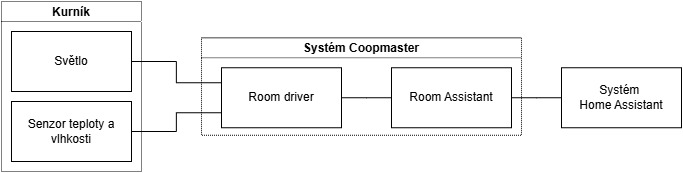
\includegraphics[width=\textwidth]{img/svetlo_teplo_vlhkost}
    \caption{Diagram ovládání světla a poskytování dat o teplotě a vlhkosti}
    \label{fig:svetlo_teplo_vlhkost}
\end{figure}

\subsection{Automatizace dvířek}
Hlavním z důvodů proč vznikl tento projekt, je zautomatizování ranního otevírání a večerního zavírání dvířek v kurníku.
V této sekci si tedy zjednodušeně popíšeme princip, jak je v systému Coopmaster řešené automatické ovládání dvířek.
Graficky jsou závislosti mezi jednotlivými moduly vysvětleny v obrázku~\ref{fig:automatizace_dvirek}.\newline
Dvířka v našem systému jsou kontrolována pomocí modulu řídící jednotka.
Room Driver zajišťuje pomocí USB sběrnice a HTTP protokolu komunikaci mezi řídící jednotkou a Room Assistantem.
Room Assistant je jak, již bylo zmíněno, propojen se systémem Home Assistant pomocí MQTT protokolu.
Dále v této sekci potřebujeme získat data z kamerového systému konkrétně z kamery v kurníku.
Komunikaci s kamerovým systémem zajišťuje přes HTTP protokol modul Camera Driver.
Tento modul má vystavené REST API a poskytuje obrázky službám v systému Coopmaster.
O obrázky si zde říká služba Chicken Watch Guard, která za pomocí neuronové sítě, konkrétně pak metody klasifikace, počítá slepice v kurníku a výsledný počet posílá opět pomocí MQTT do Home Assistanta.
Chicken Watch Guard také předává co minutu do systému Home Assistant obrázek z kamery v kurníku.
Home Assistant pro tuto sekci zajišťuje indikaci stavu dvířek, ovládací tlačítka pro dvířka, vizualizaci počtu slepic v kurníku a zobrazuje fotografii pořízenou v kurníku.
Hlavním důvodem, proč je v projektu použit Home Assistant, je jeho funkcionaliza pro automatizaci různých operací.
Zde je toho právě využito pro automatizaci zavírání a otevírání dvířek.
Home Assistant je nakonfigurován tak, aby se od určitého časového okamžiku snažil zavřít dvířka pod podmínkou, že bude počet slepic, který identifikoval Chicken Watch Guard, stejný jako ten, jež jsme nastavili jako pevnou konstantu neboli aktuální počet slepic v kurníku.
\begin{figure}[h]
    \centering
    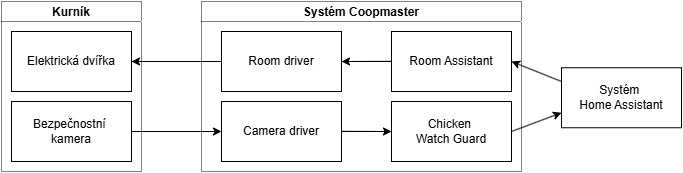
\includegraphics[width=\textwidth]{img/automatizace_dvirek}
    \caption{Diagram bezpečného zavření dvířek}
    \label{fig:automatizace_dvirek}
\end{figure}

\subsection{Detekce vetřelců}
Pro tento úkol bude třeba využít obrázků z kamery ve výběhu a umělé inteligence, která v obraze rozpozná určené vetřelce.
Princip komunikace je graficky vysvětlen v obrázku~\ref{fig:detekce_vetrelcu}.\newline
S kamerou ve výběhu komunikuje pomocí HTTP protokolu služba Camera Driver.
Z REST aplikačního rozhraní služby si stahuje obrázky služba Dog Alert.
Tato služba využívá neuronovou síť k detekci vetřelce v obraze.
Pokud je detekováno nějaké nebezpečí, služba pomocí MQTT protokolu informuje systém Home Assistant a předá mu aktuální fotografii, v níž byl vetřelec detekován jako důkaz.
Home Assistant je nastaven tak, že při přijetí takové zprávy, odešle uživateli do aplikace v mobilním telefonu oznámení, aby ho upozornil na detekci hrozby.
Dog Alarm dále pak každou minutu posílá do Home Assistanta aktuální snímek z kamery ve výběhu, aby měl uživatel stále přehled.
\begin{figure}[h]
    \centering
    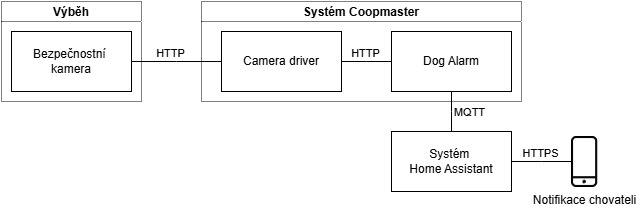
\includegraphics[width=\textwidth]{img/detekce_vetrelcu}
    \caption{Diagram detekce vetřelců}
    \label{fig:detekce_vetrelcu}
\end{figure}

\subsection{Vizualizace stavů hnízd}
Abychom splnili tento úkol, bude potřeba získat data z jednotlivých vah ve hnízdech.
Tato data pak dostat z do systému Coopmaster.
Coopmaster následně data vyhodnotí a výsledky předá k vizualizaci do systému Home Assistant.
Schémadické vyjádření principu pro vizualizaci stavů hnízd je znázorněno v obrázku~\ref{fig:vizualizace_stavu_hnizd}. \newline
Pro komunikaci s modulem digitální váhy je použita služba Scale Driver, která s jednotlivými váhami komunikuje přes USB sběrnici.
Data o váhách si ze Scale Driveru stahuje služba Nest Watcher.
Tato služba ukládá v daném intervalu data z každé váhy do databáze.
Služba po uplynutí časové konstanty analyzuje časovou řadu v databázi a vyhodnotí stav hnízda.
Detailní popis algoritmu v sekci o službě Nest Watcher (\ref{sec:nest-watcher}).
Po vyhodnocení stavů jsou data předávána pomocí MQTT protokolu do systému Home Assistant, který je díky na míru dělané komponentě zobrazí uživateli.
\begin{figure}[h]
    \centering
    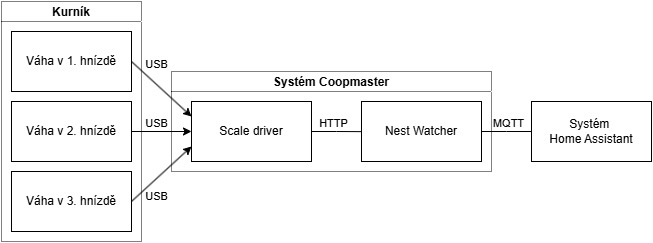
\includegraphics[width=\textwidth]{img/vizualizace_stavu_hnizd}
    \caption{Diagram vizualizace stavů hnízd}
    \label{fig:vizualizace_stavu_hnizd}
\end{figure}

\section{Zpřístupnění aplikace z internetu}\label{sec:zpristupneni-aplikace-z-internetu}
Aby systém mohl sloužit svému účelu, musí být vzdáleně přístupný.
To znamená, že server, na kterém systém poběží, musí mít veřejnou IP adresu a v ideálním případě mít tuto adresu propojenou s doménovým názvem pro snadnější použití.
Tato problematika se dá řešit několika způsoby.\newline
Jeden ze způsobů je zřízení veřejné IP adresy pro svůj server.
Toto řešení je, technicky i teoreticky náročné, protože v případě, se kterým pracujeme my, běží server na lokální síti a veřejná IP adresa tedy není přímo pro náš server, ale celou síť.
To vytváří v určitých situacích velmi vážná bezpečnostní rizika, díky čemuž je tato metoda velice náročná na hardware a implementaci.
Navíc poskytování veřejné IP adresy je placená služba poskytovatele internetového připojení.\newline
Další způsob je nasazení části systému do některého z cloudových řešení jako je Microsoft Azure nebo Amazon AWS.
Tato metoda by v podstatě vyhovovala našim požadavkům, ale pokud bychom se bavili o ceně, tak to rozhodně není levné řešení. \newline
Metoda, kterou využíváme v řešení my, je snadná, jednodušší na implementaci než zřizování veřejné IP adresy a levnější než využití cloudové služby.
Tento způsob využívá takzvané tunely neboli šifrovaná spojení.
Funguje na principu, při němž zařízení šifrovaně propojíte s veřejným serverem a tento server bude skrze sebe vystavovat službu, která běží na lokálním počítači například u nás doma.
Výhoda je, že vzdálený server disponuje kvalitním a odborně nastaveným firewalem, který zajistí dobrou ochranu našeho lokálního serveru.
Tuto službu poskytuje zdarma a bez omezení například společnost Cloudflare.
Tento způsob nejvíce odpovídá našim požadavkům, které byly cena a jednoduchost společně s rychlost nasazení.\newline
Poslední nutností, kterou ovšem je třeba zaplatit, je pronájem vlastního doménového jména.
Doménu si lze pronajmout u doménových registrátorů jako jsou GoDaddy, Hostinger nebo například Forpsi.
Ceny domén se odvíjí na základě jejího druhu a pohybují od 20 do 1500 korun za kus.
My v našem řešení využíváme službu Forpsi, protože s ní máme již předchozí zkušenost.\newline
Dále je tato část rozvedena v sekci~\ref{ch:nasazeni-systemu-do-produkce}, kde je popsán konkrétní způsob nasazení do funkčního projektu.

\newpage

\newpage
\chapter{Popis jednotlivých modulů systému}\label{ch:popis-jednotlivych-modulu}
\section{Camera Driver}\label{sec:camera-driver}
Camera Driver je služba zodpovědná za zprostředkování komunikace mezi IP kamerami a službami zpracovávajícími obraz (Dog Alarm, Chicken Watch Guard).\newline

\subsection*{Popis algoritmu}
Po startu služby naběhne REST API na portu 9001 vytvořené za pomoci Python frameworku Flask~\cite{FlaskFramework}.
Toto API poskytuje endpoint pro získání aktuálního snímku z každé kamery, která je službě přiřazena v konfiguraci modulu.
S kamerami pak služba komunikuje pomocí HTTP protokolu.
Byla zvažována i možnost využití protokolu RTSP, ale jelikož moje řešení prozatím nemá vysoké nároky na živý přenos, ukázala se jako lepší volba využití REST API kamery, které umožnuje stační aktuálního snímku na požádaní.
Jakmile je přijat požadavek na získání aktuálního snímku z konkrétní kamery, služba za pomocí GET requestu stáhne obraz z restového API síťové kamery a vrátí ho ve \gls{fullhd} rozlišení jako odpověď na HTTP dotaz.
Endpoint kamery ze kterého má služba obrázek stahovat, získá z konfigurace předávané pomocí systémových proměnných.
Kamery mají vlastní zabezpečení proti neoprávněnému přístupu k datům.
V případě ověřování HTTP komunikace se používá metoda Digest Access Authentication~\cite{digestAccessAuth}, pomocí které je kameře předáváno uživatelské jméno a heslo.


%# coopmaster-camera-driver
%- komunikator mezi IP camerou a obraz zpracovavajici aplikaci (dog alarm, chicken watch guard)
%
%## funkcionalita
%- nese si informaci o konfiguraci jednotlivych IP kamerach aktuálně je zde pevně zahardcoděne používání dvou kamer 1. pro dog alarm a 2. pro chicken watch guard
%- vystavuje REST API pro ziskani aktualniho obrazu z chicken kamery a kamery v ohrade
%- vraci obrazek ve FULL HD rozliseni
%- pro každý call se načte nový obrázek z kamery
%
%## technologie
%- python
%- rtsp - real-time streaming protocol
%- knihovny
%
%
%## hardware
%- IP camera Hilook by Hikvision IPC-B180HA-LU
\section{Scale Driver}\label{sec:scale-driver}
Scale driver zodpovídá za komunikaci mezi fyzickou váhou a službami, které využívají data o vážení.\newline

Jako řídící jednotka váhy je použito Arduino(\ref{sec:arduino}).
Scale driver modul je připojen USB kabelem a komunikuje přes sériový port.
Pomocí jednoduchého proprietálního protokolu a na přijatý dotaz poskytne jako odpověď aktuální hodnotu načtenou ze senzoru váhy.
Scaler driver má vystavené REST rozhraní, které umožnuje komunikaci s ostatními komponentami systému.

\subsection*{Popis algoritmu}
Nejprve naběhne hlavní vlákno, které se stará o poskytování REST API na portu 9004.
Toto API obsahuje endpoint pro vrázení aktuální hmotnosti na váze pomocí požadavku s metodou GET.
Následně je spuštěno nové vlákno, které má za úkol číst data z váhy a předávat je aplikačnímu rozhraní jako aktuálně naměřenou hmotnost na váze, jež se bude od teď poskytovat, pokud o ní někdo GET requestem požádá.
Čtení informací z váhy se provádí v nekonečném cyklu.
Před začátkem cyklu se do log souboru zapíše informace ohledně úspěšného spuštění nového vlákna.
Poté proběhne otevření komunikace s váhou přes seriový port s využitím knihovny PySerial.
Po úspěšném otevření spojení se váze vždy po uplynutí časového intervalu 2 sekundy, odešle znak "w".
Tento znak je ve firmwaru váhy veden jako příkaz, po jehož přijetí má váha vrátit aktuální naměřenou hodnotu.
Časové zpoždění je implementováno kvůli tomu, že není třeba číst data tak často a zároveň by mohlo docházet k zahlcení váhy.
Jakmile je celá odpověď od váhy přijata programem zpět, jsou data zvalidována a následně, pokud je to možné, převedena na datový typ Int.
Datový typ Int je zvolen z důvodu, že váha posílá data v gramech a je zbytečné v tomto případě používat desetinná čísla, protože gramy poskytují dostatečné rozlišení pro naše účely.
Pokud se nepodaří převézt přečtenou hodnotu na číslo, je výstupní proměnná nastavena na -1, což zbytku systému naznačí, že váha není v pořádku.
Na závěr se zalogují aktuálně získaná data a následuje další volání cyklu.



\section{Room Driver}\label{sec:room-driver}
Room Driver zajišťuje komunikaci mezi službou Room Assistant a řídící jednotkou v kurníku.
Tato jednotka se stará o ovládání dveří, světla a poskytování dat o aktuální teplotě a vlhkosti.
Ovládání nízkoúrovňových komponent a komunikaci s připojeným počítačem zajišťuje Arduino Nano.
Arduino je připojeno pomocí USB sběrnice k počítači, který na základě domluvených pravidel jednoduchého komunikačního protokolu posílá znaky, na které Arduino příslušně reaguje dle programu.
Tato služba má tedy za úkol přes sériové rozhraní posílat příkazy a načítat stavy řídící jednotky na základě requestů přijmutých na REST API.

\subsection*{Popis algoritmu}
Po startu služby se nejdříve vytvoří instance třídy ArduinoReader.
Jedná se o vlastní třídu, při inicializaci vytvoří instanci sériového spojení k Arduinu.
Je zde implementován connection pool, který se stará o zdraví spojení po celou dobu běhu aplikace.
Třída má jedinou metodu, a tou je run\_command.
Tato metoda přijímá jako parametr jeden znak, který při provolání metody pošle zkrze sériové připojení do Arduina a vrátí data typu String, kterými odpoví Arduino zpět.
Jakmile se povede provést inicializaci sériového spojení je spuštěno REST API.
Toto API poskytuje endpointy pro vyslání příkazů k zavření a otevření dvířek, zhasnutí a rozsvícení světla, informací o aktuálních stavech jednotky a informací o teplotě a vlhkosti v kurníku.
Informace o aktuálním stavu jsou dobré pro případ, kdy se budou muset služby restartovat a bude třeba načíst reálný aktuální stav.
V případě, kdy přijde požadavek na konkrétní endpoint, jako první věc se provede odeslání příslušného znaku jako příkaz Arduinu.
Následně se počká na jeho odpověď, pokud je požadavek typu POST.
Odpověď je následně převedena do \gls{json} objektů a vrácena v HTTP odpovědi s typem těla odpovědi JSON.

\subsection*{Příkazy ovládacího protokolu}
\begin{itemize}
    \item o = otevřít dvířka
    \item c = zavřít dvířka
    \item l = rozsvítit světlo
    \item d = zhasnout světlo
    \item j = vrátí zprávu ve formátu JSON s daty o teplotě a vlhkosti
    \item s = vrátí zprávu ve formátu SJON s daty o stavech jednotlivých ovládaných prvků (dveře, světlo)
\end{itemize}


(obrázek \ref{fig:homeasistant_temperature}).

\begin{figure}[H]
    \centering
    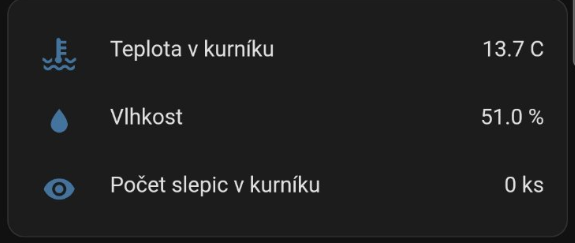
\includegraphics[width=0.8\textwidth]{img/homeasistant_temperature}
    \captionAuthorSource{Vizualizace dat ze senzoru v systému Home Assistant}
    \label{fig:homeasistant_temperature}
\end{figure}


%# coopmaster-room-driver
%
%Aplikace provazuje core aplikace(konkrétně službu room assistant) s arduinem ovladajicim svetla, dvere a poskytujici informaci o teplote a vzdusne vlhkosti.
%Součástí projektu je i firmware arduina.

%## funkcionalita
%- umoznuje ovladat osvetleni kurniku
%- resi otevírání a zavírání dvířek v kurníku
%- ziskava informace ze senzoru o teplote a vlhkosti v kurniku
%- komunikuje se zbytkem systému pomocí rest api
%- s arduinem komunikuje pomocí serialového portu a pomocí zasílání příkazů v podobě jednoho písmene
%- příkazy: o = otevřít dvířka, c = zavřít dvířka, l = rozsvítit světlo, d = zhasnout světlo, j = vrátí json s daty o teplotě a vlhkosti, s = vrátí json s daty o stavech jednotlivých ovládaných prvku (dvěře, světlo)
%
%## technologie
%- python
%- knihovny pro python
%- **Flask**: Lehký webový framework, flexibilní a rychlý vývoj webových aplikací.
%- **colorama**: Manipulace s barvami v textovém výstupu na terminálu.
%- **waitress**: Rychlý WSGI server pro produkční nasazení webových aplikací.
%- **requests**: Jednoduché HTTP požadavky (GET, POST, atd.).
%- **Werkzeug**: WSGI nástroje pro webové aplikace (routování, správa relací).
%- **python-dotenv**: Načítání konfigurace z `.env` souborů.
%- **pyserial**: Komunikace se sériovými zařízeními přes sériové porty.

\section{Health Checker}\label{sec:health-checker}
Health Checker je malá služba určená pro správce systému.
Poskytuje informace o tom, zda všechny služby běží, aby správce nebyl nucen přihlašovat se vzdáleně na server a manuálně kontrolovat každou službu.
Výpis stavů jednotlivých služeb je poskytován pomocí jednoduché webové stránky.

\subsection*{Popis algoritmu}
Po nastartování služby je spuštěno REST API na portu 9000 pro komunikaci se správcem.
Jediným endpointem služby je <server:port>/status.
Pokud uživatel pomocí prohlížeče pošle GET požadavek na tuto službu, bude mu vrácen seznam služeb a jejich stavů převedený do formátu JSON (obrázek~\ref{fig:healthchecker_report}).
Stavem aplikace je myšlen status kód a případné chybové hlášky, které služby po zavolání jejich metody <server:port>/ping.

Seznam služeb, které má Health Checker kontrolovat, je načítán z konfiguračního souboru při startu služby.
Jednotlivé služby jsou v seznamu identifikovány na základě IP adresy a portu.

Algoritmus funguje na základě plánovače úloh neboli scheduleru, který jednou do minuty spustí kontrolu všech služeb a jejich stavy uloží do seznamu odkud jsou pak načítány při požadavku na API.
Kontrola se provádí právě posláním HTTP požadavku na <server:port>/ping každé služby a následným uložením odpovědi.

Tento modul umí poskytovat základní informace o aktuálním stavu služeb sytému Coopmaster.
Pokud by se v budoucnu objevil požadavek na historická data, bylo by velmi jednoduché integrovat tuto komponentu s některou z open source platforem určenou pro analytiku a vizualizaci dat.
Například Grafana~\cite{grafana} umožňuje uživatelům vytvářet interaktivní a dynamické panely (dashboardy), které vizualizují různorodé časové řady dat získané z různých zdrojů (obrázek~\ref{fig:health-checker-grafana-dashboard}).


\begin{figure}[H]
    \centering
    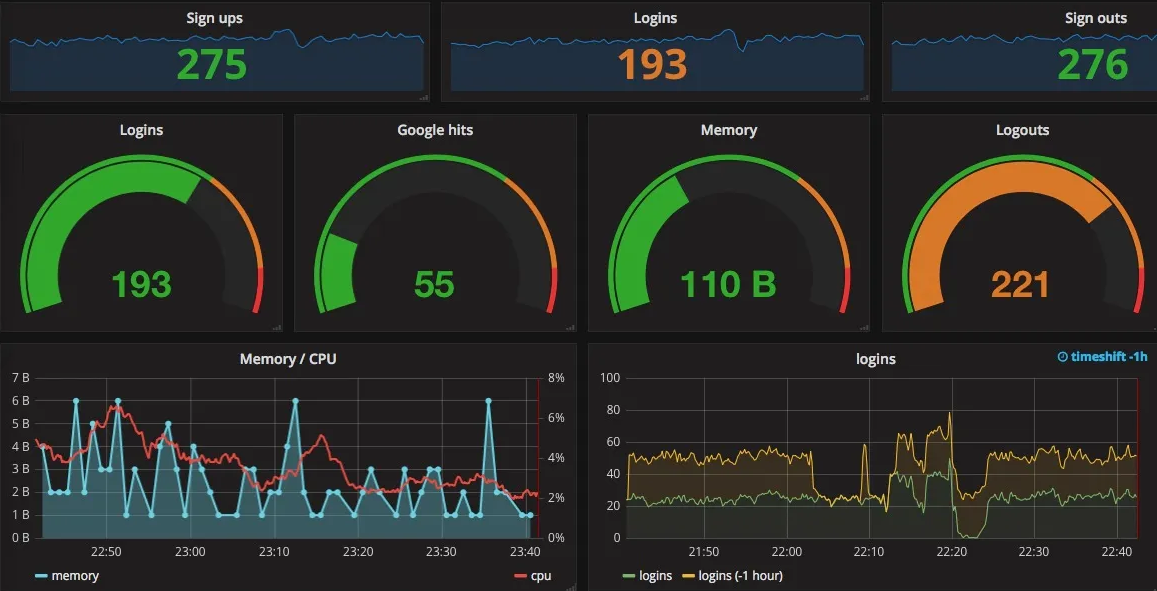
\includegraphics[width=0.8\textwidth]{img/health-checker-grafana-dashboard}
    \captionAuthorSource{Možná vizualizace pomoci platformy Grafana}
    \label{fig:health-checker-grafana-dashboard}
\end{figure}
\begin{figure}[H]
    \centering
    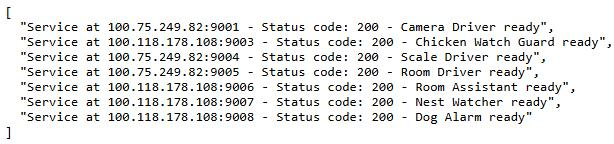
\includegraphics[width=0.8\textwidth]{img/healthchecker_report}
    \captionAuthorSource{Výstupní ze služby Health Checker}
    \label{fig:healthchecker_report}
\end{figure}
\section{Room assistant}\label{sec:room-assistant}
Room assistant zpřístupňuje komunikaci mezi systémem Home Assistant a službou Room Driver.\newline
S Home Assistantem je komunikace realizována pomocí MQTT(\ref{sec:mqtt}) a s Room driverem pomocí HTTP(\ref{sec:http-rest}) protokolu.
Tato služba zpřístupňuje do systému Home Assistant data o teplotě a vlhkosti a Home Assistant přes ní ovládá světlo a dvířka.

\subsection*{Funkcionalita}
Po odstartování služby se stane hned několik věcí.
Jako první naběhnou MQTT subscribery pro přijímání příkazů ze systému Home Assistant.
Jeden přijímá příkazy pro dívřka druhý pro světlo.
Vytvoří se vlastně instance dvou tříd LampTimeChecker a DoorTimeChecker.
Tyto instance mají každá svou instanci třídy NestMQTTClient, která zaobaluje základní funkcionalitu ohledně používání protokolu MQTT.\newline

\textbf{NestMQTTClient} zaobaluje metody pro publikování a odebírání zprávy, připojení a odpojení od MQTT brokeru, reakci na navázané spojení s MQTT brokerem a reakci na odebrání nové zprávy.\newline
\textbf{LampTimeChecker} odebírá téma coopmaster/room/lamp/cmnd a zpracovává zprávu pokud je jejím obsahem \textbf{on} nebo \textbf{off}.
Na základě přijatého obsahu zprávy se zavolá statická metoda call\_room\_driver\_command třídy driver\_client, aby odeslala příslušný příkaz do Room Driveru na endpoint, který je předáván jako parametr.

\textbf{DoorTimeChecker} funguje stejně jako NestMQTTClient, ale odebírá téma coopmaster/room/door/cmnd a reaguje pokud je obsah MQTT zprávy \textbf{open} nebo \textbf{close}.
.\newline
Po startu se rozběhne BackgroundScheduler, který má za úkol vždy po uplinutí 5 vteřin spustit nový běh jobu pro aktualizování stavů z řídící jednotky.
Podmínkou pro spuštění nového běhu jobu je, že předchozí běh musí být dokončen.
Tuto funkci má již v sobě implementovanou scheduler z knihovny APScheduler, který využíváme.
Job pro aktualizaci obsahuje jednu metodu a to detect\_hardware\_state.
Tato metoda nejdříve stáhne data z Room Driveru.
Následně načte z konfigurace témata pro stav dvíře, stav světla, teplotu a vlhkost.
Dále jsou pak data z Room Driveru zveřejněna na téma daná kofigurací odkud je přijímá systém Home Assistant a vizualizuje je.

%\subsection*{MQTT témata}
%\begin{itemize}
%    \item coopmaster/room/door/cmnd
%    \item coopmaster/room/lamp/cmnd
%    \item coopmaster/room/temperature
%    \item coopmaster/room/humidity
%    \item coopmaster/room/door/state
%    \item coopmaster/room/lamp/state
%\end{itemize}
\section{Nest watcher}\label{sec:nest-watcher}
Tato služba interpretuje stavy jednotlivých hnízd v kurníku pro Home Assistanta.
Hlavní funkcí je načítání a analýza dat z jednotlivých vah v hnízdech, která jsou reprezentována Scale Drivery.\newline
Data jsou načítána několikrát za minutu a ukládána do databáze s časovým údajem, kdy byl záznam vytvořen.
Záznam v databázi obsahuje následující sloupce:
\begin{itemize}
    \item id: Jednoznačný identifikátor záznamu v databázi.
    \item nest\_id: Identifikační číslo hnízda (v naší implementaci aktuálně 1 až 6).
    \item weight: Naměřená hmotnost v gramech pro dané hnízdo.
    \item timestamp: Čas vytvoření záznamu.
\end{itemize}
Následně se jednou za minutu vyhodnotí průměrná hodnota během posledních několika vážení.
Tento kontinuální sběr a analýza dat nám umožňuje monitorovat statistiky pro jednotlivá hnízda.
Výsledky můžeme využít například ke zlepšení podmínek chovu.
Například v případě, kdy bychom zjistili, že některé hnízdo není pravidelně navštěvováno stejně jako ostatní, znamená to, že v hnízdě je něco, co slepice pravidelně odrazuje.\newline
\newline
Na základě vyhodnocené průměrné hmotnosti jsme schopni zjistit několik případů:
\begin{enumerate}
    \item \textbf{Hnízdo je prázdné}: Pokud průměrná hmotnost nepřevyšuje 50 gramů (vzhledem k možným chybám měření), vyhodnotíme, že hnízdo je prázdné.
    V hnízdě není ani slepice, ani vejce.
    \item \textbf{V hnízdě se nacházejí vejce}: Jestliže se hodnota hmotnosti pohybuje mezi 50 a 1200 gramy, znamená to, že v hnízdě jsou pravděpodobně vejce.
    Hmotnost jednoho vejce je přibližně 50 gramů, takže počet vajec lze vypočítat vydělením celkové hmotnosti hmotností jednoho vejce.
    \item \textbf{V hnízdě sedí slepice}: Pokud je průměrná hmotnost na váze více než 1200 gramů, vyhodnotí služba, že v hnízdě sedí slepice.
    Hmotnost slepice se pohybuje kolem 1200 gramů a více.
\end{enumerate}

Obrázek~\ref{fig:weight_egg_chart_timeline} znázořňuje hodnotu hmotnosti v čase pro hnízdo s nest\_id 1.

\begin{figure}[h]
    \centering
    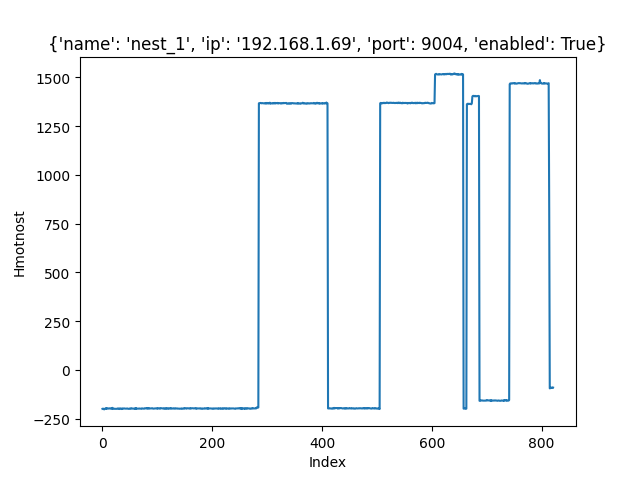
\includegraphics[width=\textwidth]{img/weight_egg_chart_timeline}
    \caption{Graf vývoje hmotnosti hnízda v čase}
    \label{fig:weight_egg_chart_timeline}
\end{figure}

Tyto tři zmíněné informace služba následně pomocí MQTT předává do systému Home Assistant, aby je zpracoval a vizualizoval chovateli.
Tím je umožněno přijímat notifikace či provádět akce na základě stavů hnízd.
Díky měřením hmotnosti z jednotlivých hnízd můžeme odvodit i další vzorce, které vypovídají o aktuálním stavu daného hnízda.
Kromě třech výše uvedených případů můžeme z nasbíraných dat identifikovat například tyto situace:

\begin{itemize}
    \item \textbf{Doba setrvání slepice v hnízdě}: Analýzou délky období, kdy je hmotnost hnízda nad 1200 gramů, lze zjistit, jak dlouho slepice v hnízdě zůstává.
    To může poskytnout informace o jejím chování, pohodě a případně upozornit na možné zdravotní problémy, pokud setrvává déle než obvykle.
    \item \textbf{Frekvence snášení u jednotlivých hnízd}: Porovnáním počtu snesených vajec v různých hnízdech lze zjistit, zda některá hnízda nejsou preferována více než jiná.
    To může vést k úpravám uspořádání kurníku nebo kontrolám hnízd, která jsou méně využívána.
    \item \textbf{Poruchy senzorů}: Pokud hmotnost zůstává nezměněna po dlouhou dobu nebo vykazuje nerealistické hodnoty, může to indikovat technickou závadu.
    Pravidelná kontrola a kalibrace senzorů zajistí spolehlivost dat.
    \item \textbf{Denní vzorce aktivity}: Analýzou hmotnostních dat během dne lze určit období nejvyšší aktivity slepic.
    To může být užitečné pro plánování krmení, čištění kurníku nebo jiných činností, které by mohly slepice rušit.
\end{itemize}

Celkově systém obsluhuje šest hnízd, přičemž se data z každého hnízda monitorují a vyhodnocují.
Toto komplexní sledování umožňuje efektivní řízení kurníku, zajišťuje optimální péči o slepice a včasný sběr vajec.
Přístup založený na datech zvyšuje naši schopnost udržovat zdravé slepice a maximalizovat jejich produktivitu.

%\subsection*{Předpokládaná datová struktura v databázi:}
%
%\begin{table}[h!]
%    \centering
%    \begin{tabular}{lll}
%        \textbf{Pole} & \textbf{Datový typ} & \textbf{Popis}                                    \\
%        timestamp     & DATETIME            & Datum a čas měření                                \\
%        nid           & INT                 & Identifikační číslo hnízda (1 až 6)               \\
%        weight        & FLOAT               & Naměřená hmotnost v gramech                       \\
%        nest\_status  & VARCHAR             & Stav hnízda (např. "prázdné", "vejce", "slepice") \\
%    \end{tabular}
%    \caption{Datová struktura v databázi}
%\end{table}
%
%Tato datová struktura umožňuje efektivní ukládání a vyhodnocování dat z jednotlivých hnízd. Pole \texttt{nest\_status} může být automaticky vypočítáno na základě hodnoty v poli \texttt{weight} podle výše uvedených kritérií. Tímto způsobem můžeme snadno filtrovat a analyzovat data pro sledování stavu každého hnízda v čase.
%
%Rozšířená analýza nám poskytuje hlubší vhled do chování slepic a umožňuje nám přijímat informovaná rozhodnutí pro zlepšení podmínek v kurníku, zvýšení produktivity a zajištění pohody zvířat.

%Data jsou načítána několikrát do minuty a ukládána do databáze s časovým údajem, kdy byl záznam vytvořen.
%Následně se jednou za minutu vyhodnotí průměrná hodnota během posledních několika vážení.
%Na základě tohoto údaje jsme schopni zjisti několik případů
%\begin{itemize}
%    \item hnízdo je prázdné (hodnota na váze nepřevyšuje 50 g )
%    \item v hnízdě se nacházejí vejce (hmotnost jednoho vejce je průměrně 50 g)
%    \item v hnízdě sedí slepice (hmotnost slepice se pohybuje okolo 1200 g a více)
%\end{itemize}
%Pokud je na váze průměrně méně než 50 g, vzhledem k možným chybám měření, takový případ vyhodnotíme jako, že je hnízdo prázdné.
%Jestliže se hodnota pohybuje mezi 50 a 1200 gramy, znamená to, že v hnízdě jsou pravděpodobně vejce, a jejich počet je vypočítán vydělením celkové hmotnosti a hmotnosti jednoho vejce.
%V případě, že je na váze více jak 1200 g, vyhodnotí služba, že v hnízdě sedí slepice.
%Tyto tři zmíněné informace služba následně pomocí MQTT předává do Home Assistanta.

\section{Dog alarm}\label{sec:dog-alarm}
Služba Dog alarm má detekovat nebezpečí ve výběhu a poslat tuto zprávu do Home Assistanta.\newline
Aktuální záběry jsou pomocí GET requestů stahovány z konkrétní instance služby Camera driver, která je přiřazena ke kameře ve výběhu.
Analýza probíhá v určitých intervalech za pomocí umělé inteligence, kde je konkrétně použita metoda detekce objektů.
Jakmile jako výsledek klasifikace vyjde jednoznačně, že v záběru byl spatřen pes nebo jiný predátor, je zpráva poslána pomocí MQTT do Home Assistanta společně s konkrétním záběrem, na němž byl predátor detekován.
Tato služba zároveň přes MQTT posílá do Home Assistanta aktuální záběr z kamery.
\section{Chicken watch guard}\label{sec:chicken-watch-guard}
Služba Chicken Watch Guard je dalším klíčovým prvkem systému Coopmaster.
Poskytuje data o počtu slepic v kurníku a tato data předává do systému Home Assistant.\newline

\subsection*{Obecný princip}
Podobně jako u služby Dog Alarm, Chicken Watch Guard používá kamerový systém pro získávání aktuálních záběrů z kurníku.
Tyto záběry jsou staženy ze služby Camera Driver~\ref{sec:camera-driver}.
Získané obrázky se analyzují modelem Yolov11, který je upravený pro přesnější detekci v našich lokálních podmínkách.
Výsledky detekce společně s aktuální fotografií jsou pomocí protokolu MQTT odeslány do systému Home Assistant, který je využije při automatizaci dvířek a vizualizuje v uživatelském rozhraní.

\subsection*{Popis algoritmu}
Jako první je vytvořeno API definované pomocí Flask frameworku pro komunikaci se službou Health Checker.
Následně je inicializován a spuštěn scheduler, který má za úkol jednou za minutu spustit job s názvem check\_chicken.
Závěrem spouštěcí metody se spustí propagace API na portu 9003, který je předáván jako proměnná prostředí při startu služby.

\subsection*{Popis algoritmu pro job check\_chicken}
Po spuštění se jako první provolá metoda get\_image, která je zodpovědná za stažení aktuálního obrázku ze služby Camera Driver.
Dále je inicializován detekční upravený model Yolov11 a provedena detekce objektů v obraze (sekce~\ref{sec:detekce-objektu-pomoci-strojoveho-uceni}).
Výsledkem je seznam objektů, které se podařilo identifikovat.
Hlavními daty, která obsahuje jedna položka v seznamu, jsou informace o detekované kategorii a oblast v obraze, kde přesně byl objekt nalezen.
Počet slepic v kurníku je dán počtem, kolikrát se v seznamu výskytuje kategorie slepice.
Job končí publikováním výsledného počtu slepic na MQTT topic coopmaster/chicken/count
 a aktuální fotografie (obrázek~\ref{fig:foto_z_guarda}) na MQTT topic coopmaster/chicken/image/actual.
Systém Home Assistant je MQTT subscriber zmíněných topics a reaguje na ně, jak je popsáno v sekci~\ref{sec:tvorba-gui-rozhrani}.

\begin{figure}[H]
    \centering
    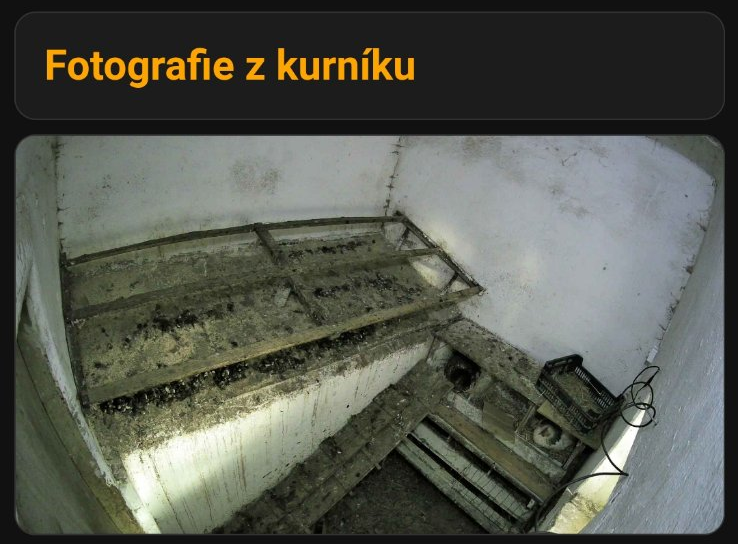
\includegraphics[width=0.6\textwidth]{img/foto_z_guarda}
    \caption{Obrázek přijatý z MQTT a vizualizovaný v dashboardu}
    \label{fig:foto_z_guarda}
\end{figure}

%\subsection*{Výhody a přínosy}
%
%Implementace služby Chicken Watch Guard přináší do systému Coopmaster následující výhody:
%\begin{itemize}
%    \item \textbf{Přesný monitoring:} Automatizovaný systém poskytuje přesné a aktuální informace o počtu slepic, což napomáhá efektivnímu plánování a rozhodování.
%    \item \textbf{Reálný čas přehledu:} Díky integraci s Home Assistanta je zajištěno promptní informování o změnách v kurníku, což umožňuje rychlou reakci.
%    \item \textbf{Vizualizace stavu:} Průběžné vizuální sledování přispívá k lepšímu porozumění a řízení prostředí v kurníku.
%\end{itemize}
%Úkolem služby Chicken watch guard je sledovat stav a počet slepic v kurníku.\newline
%Aktuální záběry jsou stejně jako u Dog alarmu stahovány z konkrétního Camera driveru v kurníku.
%Následně po získání záběru proběhne detekce objektů a počet těchto objektů udává počet detekovaných slepic v obraze.
%Tato hodnota je publikována pomocí MQTT do Home Assistanta.
%Vedlejší funkcí služby je průběžné posílání aktuálního pohledu z kamery v kurníku do Home Assistanta.

\section{Uživatelská aplikace}\label{sec:tvorba-gui-rozhrani}
Na začátku této práce jsem si v kapitole(~\ref{ch:tvorba-zadani}) identifikoval požadavky, které by měl systém Coopmaster plnit.
V této části se podíváme na funkctionalitu z pohledu uživatelského rozhraní.

Pro implementaci jsem, po prvních pokusech s vlastní aplikací, zvolil open source systém pro chytré domácnosti Home Assistant~(\ref{sec:home-assistant}).
Mezi jeho hlavní výhody patří robustnost, konfigurace, integrovatelnost a široká možnost vizualizace dat.
Vytvořit takto robustní a kvalitní uživatelské rozhraní by za mě trvalo velmi dlouho a to nepočítám čas na jeho odladění a připadné opravy.

\subsection{Požadavky na systém}

\subsubsection*{Vzdálený přístup}
Má Home Asistant podporu pro vzdálený přístup? Odpoved je ano.
Home Assistant umožňuje vzdálený přístup, což uživatelům dovoluje řídit a konfigurovat jejich chytrou domácnost odkudkoli.
Pokud se provozuje system v cloudu, je to výrazně jednodušší.
V mém případě Home Assistant běží lokálně na stroji a je přístupný pouze z lokální sítě.
Tuto drobnost jsem vyřešíl konfigurací využijeme privátního tunelu, který poskytuje například společnost Cloudflare~\cite{cloudflare}.

Podrobně je výběr technologie pro vzdálený přístup popsán v sekci~\ref{sec:zpristupneni-aplikace-z-internetu}.

Při své práci jsem systém Home Assistant využival již od začátku skrze webové rozhraní a mohu tedy potvdit, že práce s ním je příjemná a vyhovující.
Vzdáleným přístupem tedy systém disponuje a nemusíme ho tedy nijak složitě implementovat.

%todo ozdrojovat cloudflare
%todo zdroj pro mqtt image https://www.home-assistant.io/integrations/image.mqtt/

\subsubsection*{Pohledy z bezpečnostních kamer}
Zobrazování obrázků z kamer je jednou ze základních komponent, kterou HomeAssistant nabizi.
Stací si vybrat komponentu, která bude schopna zpracovat data z MQTT serveru.
Ja jsem si vybral komponentu Picture.
Použil jsem pro ni defaultní konfiguraci, jen jsem ji nastavil attribute title, abych si na dashboardu odlišil přehledová data z výbehu a kurníku.
 %todo odkaz na pouziti picture a mqtt entity pro obrázky

\subsubsection*{Dálkové ovládání a automatizaci světla a dvířek v kurníku}
Tímto bodem rozumíme v prvé řadě ovládací komponenty/tlačítka, která bude využívat chovatel, aby manuálně vyslal příkaz k provedení nějaké akce.
Za druhé se zde dostáváme k dalšímu skvělému využití systému Home Assistant a to je automatizace.
Využitím systému Home Assistant lze automatizovat právě reakce na hodnoty různých čidel a senzorů.
Může se jednat o automatizaci od úplných základů jako je zapnutí topení, když je v bytě zima, až po celé inteligentní domácnosti ovládané hlasem.
Takové domácnosti například na základě toho, kdo přišel domů, nastaví barvu světla, spustí jeho oblíbenou hudbu a uvaří kávu.
Já ve svém projektu využiji automatizaci k tomu, aby zavírala dvířka na základě času a počtu slepic, který poskytuje služba Chicken Watch Guard systému Coopmaster.
Dále pak automatizace na základě času zapíná a vypíná světlo.\newline
Pro splnění tohoto požadavku bude tedy třeba nakonfigurovat automatizaci a vytvořit ovládací tlačítka (obrázek~\ref{fig:homeassitant_lamp_button}).

\begin{figure}[H]
    \centering
    
\includegraphics[width=0.8\textwidth]{img/homeasistant_lamp_button.png}
    \caption{Komponenta pro ovládání světel systému Home Assistant}
    \label{fig:homeassitant_lamp_button}
\end{figure}


%todo přidat odkaz na coopmaster a chicken guarda a na dokumentaci home assistant automatizace

\subsubsection*{Intuitivní vizualizace stavů jednotlivých hnízd(sedící slepice, v opačném případě počet vajec)}
Tento bod je ze všech nejnáročnější.
Home Assistant totiž nedisponuje žádnou pěknou komponentou přímo pro vizualizaci hnízd v kurníku a ani žádnou jinou, která by se dala po nějakých úpravách využít.\newline
Z tohoto důvodu bude tedy třeba vytvořit vlastní komponentu pro systém Home Assistant, která půjde snadno parametrizovat dle požadavků kurníku a bude umět zpracovat data, která přijdou ze služby Nest Watcher systému Coopmaster.

\subsubsection*{Upozornění na detekování vetřelce ve výběhu}
Zde se bude opět jednat o automatizace.
Požadavkem je, aby v případě poplachu systém poslal notifikaci chovateli a zobrazil na dashboardu aktuální fotografii, kde byl vetřelec detekován.\newline
Abychom splnili tento bod, budeme muset nastavit automatizaci, která zareaguje na určitý stav nějaké MQTT entity a následně vytvoří notifikaci.
Tato notifikace vyskočí i na chovatelově telefonu.
Dále bude použita komponenta s názvem Conditional, která umožnuje na základě hodnoty, měnit vizualizaci komponent na dashboardu.
Pri určitém stavu MQTT entity zobrazí v dashboardu upozornění na vetřelce ve výběhu a opačném případě nezobrazí nic.
Což je velmi šikovné právě pro různá upozornění.
%//todo odkaz na komponentu conditional

\subsubsection*{Data o teplotě a vlhkosti}
Tyto dva požadavky nebudou, co do implementace nic složitého.
Jedná se pouze o dvě hodnoty, které navíc ze služby Room Assistant chodí ve formátu JSON, takže není problém je zpracovat.\newline
Bude tedy třeba jen nakonfigurovat MQTT entitu, kterou následně bude načítat komponenta Entities.
Tato komponenta zobrazuje v seznamu pod sebou entity, jejichž seznam přebírá jako parametr.
Pro zobrazení každé entity je možno upravit ikonu a zobrazovaný název, což přesně odpovídá našim požadavkům.
%todo odkaz na kompoentu entities

\subsection{Postup konfigurace systému Home Assistant}
Po rozvržení řešení jsem se začal seznamovat se systémem Home Assistant s čímž mi hodně pomohla rozsáhlá a kvalitní dokumentace společně s diskusními fóry, která jsem hojně využíval.
\subsubsection*{MQTT entity}
Konfiguraci jsem započal definováním všech potřebných MQTT entit v souboru configuration.yaml, do kterých systém ukládá data přijatá z MQTT brokeru a následně je můžeme využít v našem dashboardu.
Používám tři typy MQTT entit.
\begin{itemize}
    \item sensor - přijímá běžné hodnoty senzoru jako čísla a texty (maximální velikost je 255 bytů)
    \item image - umožňuje přijmout obrázek z MQTT brokeru
    \item binary\_sensor - na základě nakonfigurovaných hodnot je jeho stav buď 0 nebo 1
\end{itemize}
Každá MQTT potřebuje nastavit jednotnačné jméno pro identifikaci v systému a topic, ze kterého bude odebírat zprávy.

%todo ukazka na konfiguraci entit a na dokumentaci

\subsubsection*{Základní dashboard}
Jakmile se nakonfigurují entity, následuje tvorba samotného dashboardu.
Za pomocí webového rozhraní jsem tedy přidal tlačítka, vizualizace obrázků a výpisy hodnot entit tak, jak bylo rozebráno dříve v návrhu.
Po přidání komponent bylo třeba přiřadit odpovídající entity ke komponentám opět s využitím webového rozhraní.

\subsubsection*{Automatizace}
Díky intuitivnímu webovému rozhraní systému není problém přidat jakoukoli automatizaci.
Automatizaci si lze představit stejně jako klasickou podmínku v programování.
Je zde sekce Spouštěč, která nastavuje hlavní důvod spuštění automatizace.
Následuje volitelná sekce A Pokud.
Tato sekce udává další omezení pro spuštění scriptu.
Na závěr je zde sekce Pak Provést, která právě specifikuje akci nebo akce, které se mají uskutečnit při splnění podmínek.
S těmito vědomostmi jsem opět nakonfiguroval dle návrhu potřebné automatizace pro světlo, dvířka a notifikace.

%todo najít návod na přidávání automatizace a dat ho taky jako zdroj

\subsubsection*{Tvorba vlastní Home Assistant komponenty}
Zde se již dostáváme k opravdovému programování. Inspirací jak komponentu vytvořit mi byla developerská dokumentace~(\cite{homeassistant-developers}).
Služba Nest Watcher poskytuje data o tom zda je hnízdo obsazené a kolik je v každém hnízdě vajec.
Tato data jsou ve formátu CSV, kdy každý prvek v poli znamená jedno hnízdo.
Data se do komponenty dostávají z entit.
Tyto entity se nastavují jako parametry během přidávání komponenty na dashboard.
Data, která dostaneme z entity, jsou v CSV formátu, takže se pomocí funkce split rozdělí podle separátoru, kterým je v tomto případě znak středníku.
%todo dodat ukázky kodu
Skript pokračuje do další části, kde dochází ke zpracování naparsovaných dat.
Jednoduchými dvěma for cykly se zajišťuje vykreslování nastaveného počtu řádků a sloupců v kurníku.
Jedno hnízdo se vykresluje obarvený DIV a jeho child komponenta je DIV, který slouží k vizualizaci stavů hnízda.
Graficky jsou DIVy nastylovány tak, aby uživateli připomínali hnízdo.
Do child divu se následně vykreslí vpravo dole počet vajec, pokud je větší než 0, a zároveň se ve středu vykresluje ikonka slepice, která značí, že slepice sedí v hnízdě. (obrázek~\ref{fig:homeassitant_custom_component})
Komponenta také při každém updatu dat loguje do konzole pro případ, kdy by se něco pokazilo.

\begin{figure}[H]
    \centering
    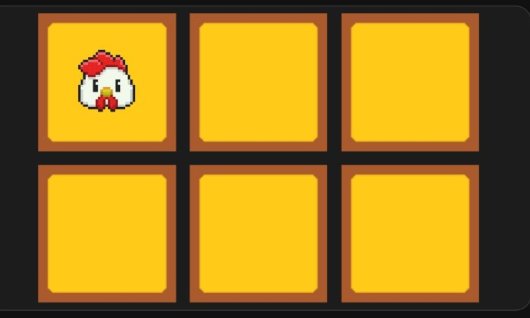
\includegraphics[width=0.8\textwidth]{img/homeassitant_custom_component}
    \caption{Vlastní komponenta pro systém Home Assistant}
    \label{fig:homeassitant_custom_component}
\end{figure}



%\subsection*{Problémy a poznatky během konfigurace}
%Během práce se systémem Home Assistant, jsem posbíral několik poznatků a narazil na několik problém.

\subsection*{Maximální velkost hodnoty senzoru}
Během tvorby komponenty pro hnízda, mě poněkud zaskočil fakt, že maximální velikost hodnoty state v entitě je 255 bytů.
Z počátku jsem chtěl posílat data o hnízdech ve formátu JSON.
Dlouho mi to procházelo, ale problém začal v situaci, kdy jsem serializoval celý seznam s objekty hnízd a chtěl ho poslat jako hodnotu senzoru.
Nebylo jednoduché na to přijít, protože v tomto případě Home Assistant data prostě nenačítal a já nevěděl proč.
Nakonec jsem se na diskusním fóru dočetl, že velikost hodnoty state je omezena.
Byl jsem tedy donucen začít používat formát CSV a posílaná data omezit pouze na nejnutnější informaci o stavu.
Pořád je zde problém s maximální velikostí v případě, že bych měl více než 128 hnízd, místo by mi i tak nevystačilo,
Na kontrolu tolika hnízd, bych ale potřeboval pravděpodobně o dost celkově robustnější infrastrukturu systému Coopmaster, takže to ponechávám ve formátu CSV.
%todo najít zdroj pro 255 bytů

%\subsubsection{Pozitivní zkušenost s tvorbou komponent}
%Práce na komponentě pro vizualizaci hnízd mi přinesla mnoho informací



\section{Digitální váha do hnízda}\label{sec:digitalni-vaha-do-hnizda}
Pro účely projektu bylo potřeba postavit digitální váhu.
Tato váha má být umístěna v každém hnízdě v kurníku, kde slepice snáší vejce, a jejím úkolem je přes USB poskytovat aktuální data o tom jakou hmotností je zatěžována podložka hnízda.

\subsection*{Popis algoritmu}
Po připojení napájení k Arduinu, se nejdříve nastaví a připojí sériová komunikace rychlostí 9600 baudů pomocí USB.
Následně je instancován objekt starající se o sprostředkování komunikace s převodníkem HX711 a nastaví se jednotlivé piny dle fyzického zapojení převodníku.
Dále je nastaven kalibrační faktor, což je konstanta používaná knihovnou HX711.h při převodu dat získaných z převodníku na gramy, s nimiž program již nadále pracuje a následně je posílá po sériovém připojení.
Jako poslední krok v rámci přípravy programu je vynulování váhy pomocí metody tare(), která je jedna z metod HX711.h knihovny.
Jakmile program dokončí fázi příprav, vstoupí do nekonečného cyklu.
Tento cyklus pravidelně čte data přicházející po seriovém připojení.
V případě, kdy jsou přijata data, program počítá se třemi scénáři.
Buď je přijat znak "w", znak "t" nebo jakákoli jiná data.
V případě znaku "w" (od slova weight) program reaguje odesláním aktuální naměřené hodnoty váhy po sériovém připojení jako reakce na příkaz.
Přijmutý znak "t" znamená tare neboli vynulovat váhu.
Na základě toho se programu řekne, že aktuální data přijímaná ze senzoru má brát jako hmotnost 0 g.


\subsection*{Konstrukce váhy}
Jako řídící jednotka váhy je použito Arduino Nano, jež je zodpovědné za komunikaci s počítačem pomocí sériového připojení a načítání dat o hmotnosti z AD převodníku HX711 přes, který je arduino připojeno k tenzometrickému senzoru.
Hmotnost je měřena tenzometrickým senzorem se jmenovitým zatížením 20 kg.
Toto zapojení je nutné vzhledem ke konstrukci a vlastnostem senzoru.
Tenzometrické senzory jsou analogové a jejich výstupem jsou velmi malé změny v napětí v rozmězí 0.15 až 1 mV.
Tyto signály jsou navíc hodně slabé, proto je nutné použít konkrétně převodník HX711, který signál zesílí a zajistí větší rozlišení díky vysoké citlivosti.
Složitější zapojení není jedinou nevýhodou.
Značnou nevýhodu představuje také fakt, že už vlivem zatížení se profil senzoru mírně deformuje a na základě toho narůstá chyba měření v průběhu času.
Tento problém se dá snadno řešit pravidelným nulováním v případech, kdy zrovna senzor zatížen není.
Na konstrukci váhy je velmi zajímavý tvar a důvody samotné železné konstrukce.
Protože má být váha instalována do již existujícího hnízda a slepice bude vlastně sedět rovnou na váze, je třeba navrhnout konstrukci váhy tak, aby slepice se funkce a způsob sezení nezměnil.
Nakonec je jako platforma, na které slepice sedí, zvolena čtvercová miska o rozměrech odpovídající s rezervou rozměrům celého hnízda.
Nemohla by to být například pouze rovná deska, protože slepice potřebuje pro pohodlné sezení podestýlku kterou tvoří seno a v případě desky by se seno dostalo mezi stěny hnízda a desku a váha by se tak nemohla volně pohybovat a zasekávala by se.
Takto v misce je mnohem menší šance, že bude nějak větší množství sena vytlačeno a bude přidírat váhu.

\subsection*{Kalibrace}
Po fyzickém sestavení váhy je třeba provést kalibraci.
Kalibrace používaných senzorů je nutná, protože se díky ní eliminují rozdíly mezi senzory, překryjí se nedostatky konstukce váhy a zajistí přesnost a korektnost měření pro konkrétní senzor.
To znamená najít vhodnou hodnotu kalibračního faktoru, která se již za běhu váhy nebude měnit.
Doporučená metoda jak provádět kalibraci, je vzít si předmět o němž víme přesně jeho hmotnost a ten použít jako vzorové závaží, na které chceme váhu kalibrovat.
Konkrétně u námi použitého senzoru do 20 kg je dobré volit závaží v řádech minimálně několika kil.
Já doma použil 5 balíčků polohrubé mouky jejichž hmotnost jsem si ověřil přesnou kuchyňskou váhou.
Následujícím krokem je nalezení odpovídající hodnoty kalibračního faktoru, čehož je docilováno buď zvyšováním nebo snižováním kalibračního faktoru na základě toho zda výsledná hmotnost dle výpočtů s využitím aktuálního faktoru je moc nízká nebo moc vysoká.


\subsection*{Hardware}
\begin{itemize}
    \item Arduino Nano v3.0
    \item AD převodník HX711
    \item Tenzometrický senzor se jmenovitým zatížením do 20 kg
    \item Železná konstrukce váhy
\end{itemize}

\subsection*{Arduino knihovny}
\begin{itemize}
    \item Arduino.h - základní Arduino knihovna
    \item HX711.h - pro usnadnění komunikace s AD převodníkem HX711
\end{itemize}

%- vysvětlit přijimane commandy w - dej vahu a t - tare
%zastrcim arduino do elektriky
%rozběhne se loop
%z pinů xy čteme hodnoty
%knihovna zpracovava hodnoty odporu
%knihovna řeší vynulování váhy
%vysvětlit kalibraci
%najít a popsat kalibrační program a vysvětlit k čemu je potřeba
%loop čeka a kontroluje serialovy vstup zda neni pismenko w nebo t
%popis loopu

%je tam převodník pro převod analogu na digital
%odecita odpor
%na konci toho je tenzometrikej můstek
%specifikace senzoru
%plusy a mínusy senzoru deformace, vysvětlit princip

%tenzometricky sezor podobne jako u vcel
%hezky popsano v praci
%uvaha o tom co vybrat zavesna vaha nebo tlacna vaha
%problemy pri implementaci
%problémy s konstrukcí a nekvalitními součástkami
%senzory se deformují a tím vzniká chyba v měření
%chyby vznikají díky analogu i chybami / odpory v elektrickém
%vedení (pevné / pájene spoje vs odnímatelné konektrory)

%knihovny arduina
%defaultní Arduino.h
%HX711.h: knihovna pro komunikaci s module AD Převodníku 24-bit 2 kanály HX711
\section{Řídící jednotka}\label{sec:ridici-jednotka}
Řídící jednotka je vlastní sestavené zařízení, které zprostředkovává pomocí USB připojení data o teplotě a vlhkosti v kurníku.
Další úlohou je ovládání dvířek a světla.
Srdcem řídící jednotky je Arduino Nano.
Tento programovatelný mikrokontroler slouží jako logický prvek mezi nízkoúrovňovými prvky (relé, senzory, táhlový motor) a počítačem.
Na počítači zase běží služby ovládající nebo využívající data z těchto prvků.

\subsection*{Popis zapojení}
Zapojení řídící jednotky je zdokumentováno na obrázku~\ref{fig:ridici_jednotka} a blokové schéma zapojení je na obrázku~\ref{fig:schema_ridici_jednotky}.

Základní komponenty řídící jednotky:
\begin{itemize}
    \item mikrokontroler Arduino Nano v3.0
    \item senzor DHT11 pro teplotu a vlhkost
    \item relé s napětím cívky 5 V a spínacím proudem 10 A stejnosměrných
\end{itemize}
Pro snadnou práci s jednotlivými součástmi během vývoje, byly zvoleny moduly, které disponují svorkovnicemi a není tedy nutné k nim nic pájet.
Připojení Ardruina je realizováno pomocí terminal schieldu, který pro každý pin desky disponuje jednou svorkou pro připojení kabelu.
Obdobně byl pro práci s relátky vybrán modul, který již 4 rele obsahoval a pro snadné zapojení také svorkovnici.

Nejkomplikovanější byl modul snímače, ke kterému bylo třeba vytvořit konektor, protože disponoval pouze výstupními piny.
Jako instalační platformu jsem zvolil dřevotřískovou desku a na ni jsem připevnil všechny moduly pomocí krátkých vrutů do dřeva.
Jednotlivé moduly byly následně propojeny vodiči o průřezu 0,15 mm² dle technické dokumentace dodávané ke každému modulu.
Hardwarová stránka byla tímto hotová.
\newline
Arduino a ostatní periferie se napájí skrze USB port Arduina, takže nebylo třeba řešit žádné přídavné napájení.
Přídavné napájení by bylo třeba řešit například, kdybychom používali 10 relejových modulů současně, protože limit pro napájení skrze USB 2.0 je pouze 500 mA~\cite{USB20proud} a jedna cívka spotřebuje až 70 mA.\newline
Následovala tedy poslední věc a to nahrát kód programu do samotné vývojové desky Arduino Nano.
Zde je výborným pomocníkem vývojářský nástroj Arduino IDE~\cite{arduino-ide}, který celý složitý proces nahrávání vyřeší.


\begin{figure}[htbp]
    \centering
    % První řádek
    \begin{minipage}[H]{0.8\textwidth}
        \centering
        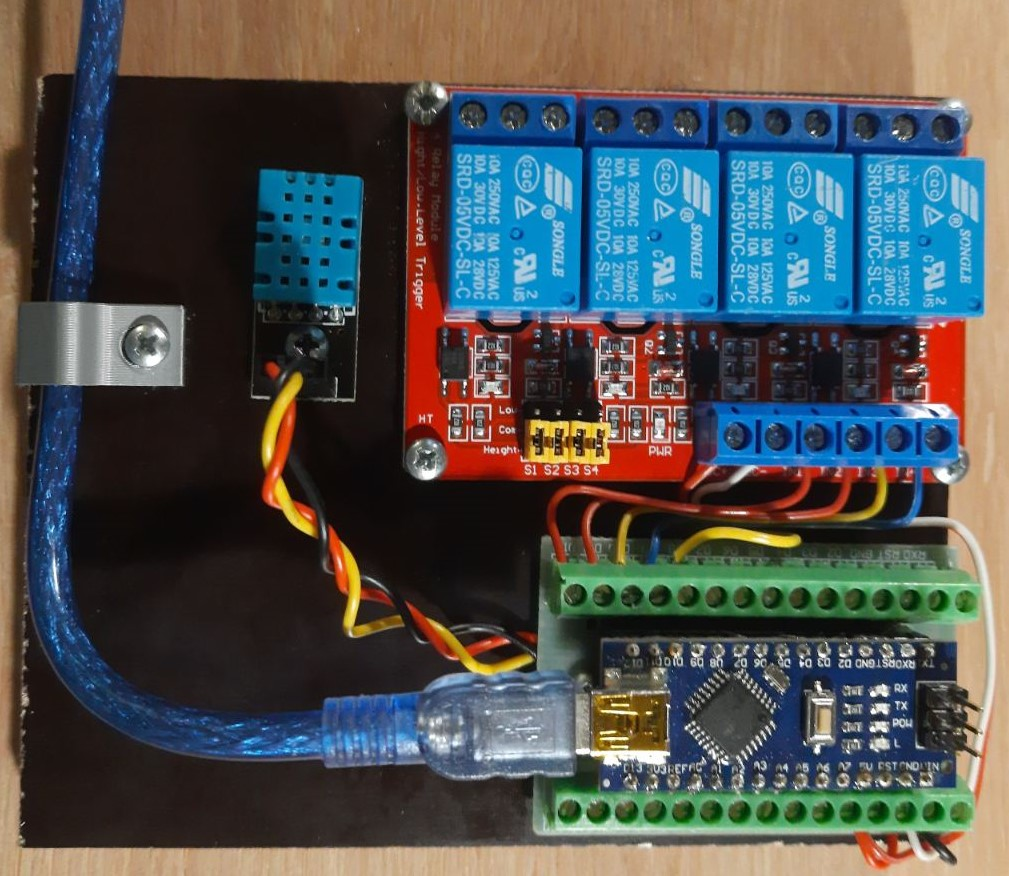
\includegraphics[width=0.8\textwidth]{img/ridici_jednotka}
        \captionAuthorSource{Skutečné zapojení řídící jednotky}
        \label{fig:ridici_jednotka}
    \end{minipage}
    \begin{minipage}[H]{0.8\textwidth}
        \centering
        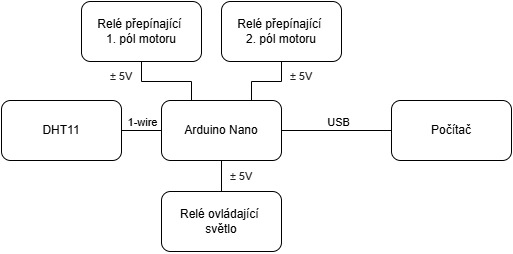
\includegraphics[width=1.0\textwidth]{img/schema_ridici_jednotky}
        \captionAuthorSource{Blokové schéma řídící jednotky}
        \label{fig:schema_ridici_jednotky}
    \end{minipage}
\end{figure}

\subsection*{Popis algoritmu}
V části programu Setup se jako první po startu programu nastaví příslušné módy na vstupní a výstupní piny.
Následně se provede inicializace sériového připojení s rychlostí 9600 baudů.
Poté se inicializuje připojení s čidlem DHT11~\cite{DHT11Datasheet} pomocí knihovny DHT.h a na závěr jsou nastaveny výstupy dle aktuálních stavů řídících neboli stavových proměnných pro dvířka a světlo.
Dále program pokračuje do části Loop, což je metoda, která se volá pořád dokola jako nekonečný cyklus.
Tato metoda řeší pravidelnou aktualizaci dat ze senzoru, dále čtení příkazů ze sériového připojení a posílání odpovědi na ně.
Aktualizace senzorových dat se provádí jednou do vteřiny za pomocí metod readTemperature a readHumidity, které jsou součástí knihovny DHT.h.
Zpracování příkazů probíhá zavoláním metody processCommand, která pokud je v zásobníku přijatých dat něco ke čtení, přečte první znak a ten následně zpracuje jako příkaz dle seznamu uvedeném v části~\ref{sec:room-driver}.
%
%\subsection*{Seznam příkazů ovládacího protokolu}
%\begin{itemize}
%    \item o = otevřít dvířka
%    \item c = zavřít dvířka
%    \item l = rozsvítit světlo
%    \item d = zhasnout světlo
%    \item j = vrátí JSON s daty o teplotě a vlhkosti
%    \item s = vrátí JSON s daty o stavech jednotlivých ovládaných prvku (dveře, světlo)
%\end{itemize}




%## funkcionalita
%- umoznuje ovladat osvetleni kurniku
%- resi otevírání a zavírání dvířek v kurníku
%- ziskava informace ze senzoru o teplote a vlhkosti v kurniku
%- komunikuje se zbytkem systému pomocí rest api
%- s arduinem komunikuje pomocí serialového portu a pomocí zasílání příkazů v podobě jednoho písmene
%- příkazy: o = otevřít dvířka, c = zavřít dvířka, l = rozsvítit světlo, d = zhasnout světlo, j = vrátí json s daty o teplotě a vlhkosti, s = vrátí json s daty o stavech jednotlivých ovládaných prvku (dvěře, světlo)
%
%## technologie
%- c++ / wire (jazyk pro programování v arduino ide)
%- knihovny pro arduino
%- defaultní **Arduino.h**
%- **DHT**: pro ovládání teplotních+vlhkostních sezorů DHT11 a DHT22
%- táhlový motor 12v nevím kolik neutonů
%- zpřevodovaný motorek k navijáku
%- relé 5v 10A
%
%
%## hardware
%- arduino Nano v3.0
%- teplotni a vlhkosti senzor DHT11
%- relatko ovladajici svetlo a relátka udávající chod a směr motoru
%- napájeno připojením ke raspberry pi přes usb napětím 5V
%
\section{Kamerový systém}\label{sec:kamerovy-system}
Kamerový systém je jeden z hlavních prvků systému Coopmaster.
Data z jeho kamer využívají skrze službu Camera driver služby Dog Alarm a Chicken Watch Guard.
Do systému jsou aktuálně instalovány dvě kamery jedna pro venkovní výběh druhá pro pohled do kurníku.
Po pečlivém výběru a volbě parametrů jsou vybrány kamery značky Hikvision typ Hilook IPC-B180HA-LU.

\subsection*{Výběr kamery}
Klíčové vlastnosti pro výběr našich kamer byly
\begin{itemize}
    \item Možnost venkovní instalace
    \item Připojení kablelem
    \item Volitelně oba způsoby napájení buď POE nebo přímo ze sítě (záleží na způsobu instalace a umístění)
    \item Kvalitní noční vidění
    \item Velké zorné pole
    \item Vysoká kvalita obrazu (dostatek dat pro umělou inteligenci)
\end{itemize}
Snažil jsem se vybrat kameru, která bude relativně cenově dostupná a bude vyhovovat zmíněným parametrům.
Musel jsem se kvůli tomu dovzdělat v mnoha ohledech, například detailně prozkoumat technologii PoE, digitálního videa, konstrukcí venkovních elektrických zařízení a mnoha dalších parametrů, které venkovní IP kamery mají.
S výsledným výběrem jsem velmi spokojený.
Kamera poskytuje kvalitní data pro vývoj tohoto systému a práce s ní není nijak komplikovaná jak je detailněji popsáno v sekci o službě Camera driver.

\subsection*{IP camera Hilook by Hikvision IPC-B180HA-LU}
Klíčové parametry, které využíváme v projektu, jsou
\begin{itemize}
    \item Rozlišení 8 Mpx
    \item Přísvit pomoci bílou LED a IR LED s dosahem až 30 m
    \item Zajímavá technologie ColorVu pro snímání barev za horších světelných podmínek
    \item Technologie Motion Detection 2.0 pro detekci osob či vozidel
    \item Technologie WDR pro zmenšení rozdílů při různě silném osvětlení scény
    \item Napájení pomocí PoE nebo přes síťový adaptér na 12V 2A.
    \item REST API a HTTP nebo RSTP protokol pro poskytování obrázků, streamování videa a zvuku
    \item Dobře zpracované webové rozhraní pro konfiguraci
\end{itemize}

%- vraci obrázek ve FULL HD rozliseni
%- pro každý call se načte nový obrázek z kamery
%
%## technologie
%- python
%- rtsp - real-time streaming protocol
%- knihovny
%
%
%## hardware
%- IP camera Hilook by Hikvision IPC-B180HA-LU
\section{Konstrukce dvířek}\label{sec:konstrukce-dvirek}
Elektrická dvířka systému Coopmaster jsou tím hlavním důvodem proč tento projekt vůbec vznikl.
Prozatím se jedná o prototyp vlastní konstrukce, který se bude před trvalou instalací ještě zdokonalen a konstrukce bude navržena vzhledem k ceně řešení a na míru potřebám chovatele.
Aktuálně jsou dvířka sestavena ze standardních hliníkových profilů.
Pro pohyb dvířek se pro prototyp jeví jako nejsnažší volba táhlový motor.
Tento motor je připevněn ke kovovému plátu, který slouží jako posuvná dvířka.
Toto řešení je nejjednodužší na realizaci, díky snadno proveditelné konstrukci.
Řešení však není ideální pro velkovýrobu, protože hliníkové součásti společně s motorem jsou příliš drahé a je zbytečné si do kurníku instalovat dvířka, která svou cenou převýší cenu vajec, které spotřebujete za rok.

Finálním řešením by se mělo
\subsection*{Táhlový motor}
Jedná se o motor, jehož součástí je samotný elektromotor a k němu je připevněn šnekový převod do síli.
Šnek je pevně upevněn na šroubovici, která se stará o rozvod síli a točivého momentu po celé délce motoru.
Převod z otáčivého pohybu na pohyb přímočarý je zajištěn maticí, která pevně drží na táhlu.
Rozhodnutí zda se bude táhlo zasouvat nebo vysouvat je dáno polaritou napětí dodávaného elektromotoru, který se na základě toho otáčí buď po nebo proti směru hodinových ručiček.

%todo obrazek dvirek
konstrukce dveri - expoziční
- přímočarý motor s dorazy
- konstrukce z hliníkových profilů a smontnotváno pomocí běžných spojovacích prvků pro práci s těmito profily
- dvířka reprezentována hliníkovým plátem tahaným lankem připěvněným k ramenu který vynáší sílu od motoru k dvířkům
- zdroj 12V
konstrukce dveri - instalováno
- zdroj 12V
- rám z železných U profilů použitých jako vodící lišty pro posuv dvířek z plastové desky a pásků které konstrukci udžují po kupě
- naviják je s dvířky přopojen lankem
- navijecí systém / systém navijáku
- 12V motor s převodovkou, rychlostí otáčení 60rpm
- navíjecí buben vytištěný na 3d tiskárně
- dorazový systém

\newpage
\chapter{Učení Yolo modelů}\label{ch:uceni_yolo_modelu}
\section{Klasifikace objektů pomocí strojového učení}\label{sec:klasifikace-objektu-pomoci-strojoveho-uceni}

\subsection{Úvod do problematiky}\label{subsec:uvod-do-problematiky}
V posledních letech došlo k významnému pokroku v oblasti strojového vidění, což umožňuje efektivní a přesné rozpoznávání objektů v různých prostředích.
Jednou z nejmodernějších knihoven, která si získala širokou popularitu, je YOLOv8 (You Only Look Once version 8).
Tato knihovna přináší rychlé a přesné metody detekce objektů a je ideální pro implementaci v reálném čase.
V této sekci se zaměříme na to, jak využít YOLOv8 ke specifickému úkolu: rozpoznávání slepic v kurníku.
Automatizované rozpoznávání umožňuje sledování počtu slepic.
Použití YOLOv8 přináší následující výhody:

\begin{enumerate}
    \item Rychlost a Přesnost: YOLOv8 je navrženo pro rychlou detekci objektů s vysokou mírou přesnosti, což je ideální pro aplikování v reálném čase na farmách.
    \item Jednoduchost Implementace: Díky snadnému rozhraní a rozsáhlé dokumentaci je integrace YOLOv8 do existujících systémů velmi přímočará.
    \item Flexibilita: Můžete trénovat model na vlastním datasetu slepic, což zajistí optimální rozpoznávání i v specifických podmínkách vašeho kurníku.
\end{enumerate}
V následujících sekcích si podrobně projdeme kroky, jak připravit dataset, trénovat vlastní model se zaměřením na rozpoznávání slepic a jak jej implementovat do našeho systému monitorování.

\subsection{Obrázkový dataset}\label{subsec:obrazkovy-dataset}

Obrázkový dataset je strukturovaná kolekce obrazových dat, která se používána pro potřeby strojového učení a počítačového vidění.
Tyto datasety obsahují jednotlivé obrázky, které jsou často spojeny s dodatečnými informacemi nebo anotacemi, jež jsou potřebné pro trénink modelů.
Níže jsou uvedeny hlavní aspekty, které charakterizují obrázkové datasety:

\begin{enumerate}
    \item Obrázky: Základní komponentou datasetu jsou samotné snímky, které mohou být v různých formátech (např. JPEG, PNG). Rozlišení a počet barev se může lišit v závislosti na účelu datasetu.
    \item Anotace: Kromě samotných obrázků obsahují datasety take anotace. Tyto anotace zahrnují následující informace
    \begin{itemize}
        \item Klasifikační štítky: Které identifikují, co se na obrázku nachází (např. „kočka“, „pes“, „slepice“).
        \item Ohraničující boxy: Které označují polohu specifických objektů na obrázku.
    \end{itemize}
\end{enumerate}

Datasety jsou klíčové pro vývoj a zlepšování modelů strojového učení, protože poskytují potřebné tréninkové a testovací údaje.
Příklady známých obrázkových datasetů zahrnují ImageNet, COCO (Common Objects in Context), a MNIST (pro ručně psané číslice).
V kontextu využití datasetů pro strojové učení je důležité zajistit, aby datasety byly kvalitní, rozmanité a dostatečně rozsáhlé, což pomáhá modelům převážně se zobecněním a výkonem v různorodých situacích.
Pro specifické nasazení v babičině kurníku jsem připravil vlastní dataset, který jsem použil pro doučení již existujícího základního modelu, který poskytuje Yolov11.
Záběry jsem vyfotil mobilem v prostředí babiččina výběhu a kurníku.
Existuje mnoho systému pro tvorbu anotaci anglicky image labeling.
Já jsem zvolil Azure AI - Azure Machine Learning studio.
Pro práci je velmi intuitivní a nechá spustit v několika krocích.
Nejdříve jsem pomocí průvodce vytvořil nový projekt jak je znázorněno na obrázku~\ref{fig:create_learning_project}.

\begin{figure}[h]
    \centering
    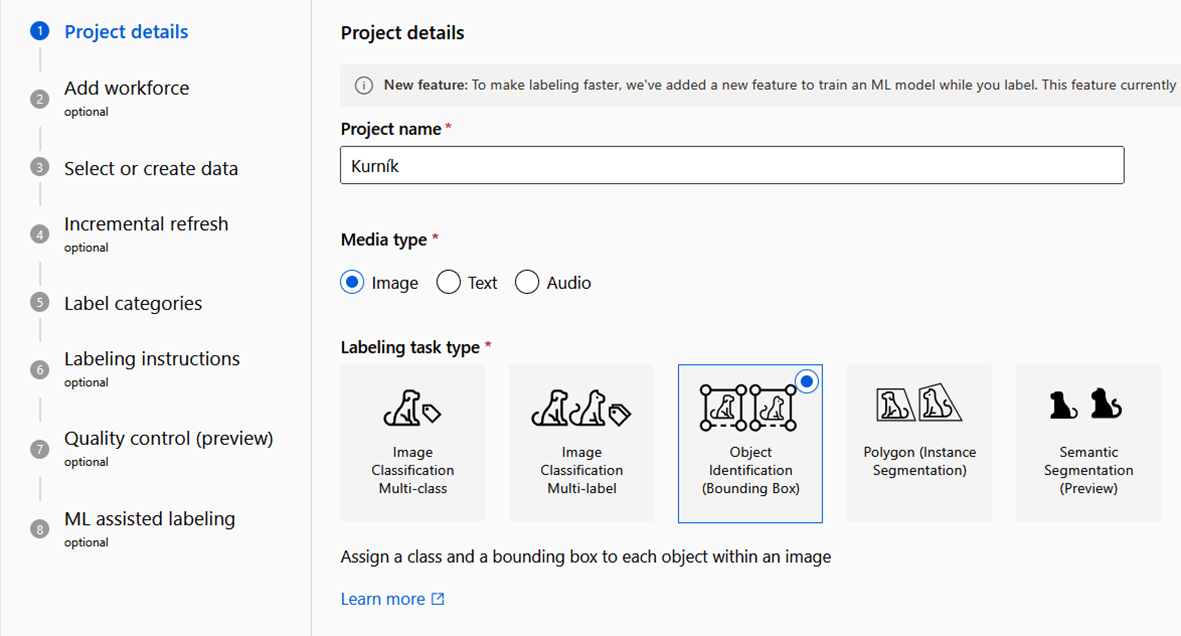
\includegraphics[width=\textwidth]{img/create_learning_project}
    \caption{Vytvoření nového projektu v AML}
    \label{fig:create_learning_project}
\end{figure}


Dále jsem vybral zdroj obrázků, které bylo potřeba klasifikovat.
Vzhledem k tomu, že se jedná o cloudovou službu bylo třeba obrázky slepiček na Azure naimportovat.
Na obrázku~\ref{fig:dataset_selection} je screenshot z Azure Machine Learning studia, kde se zrovna dataset importuje.

\begin{figure}[h]
    \centering
    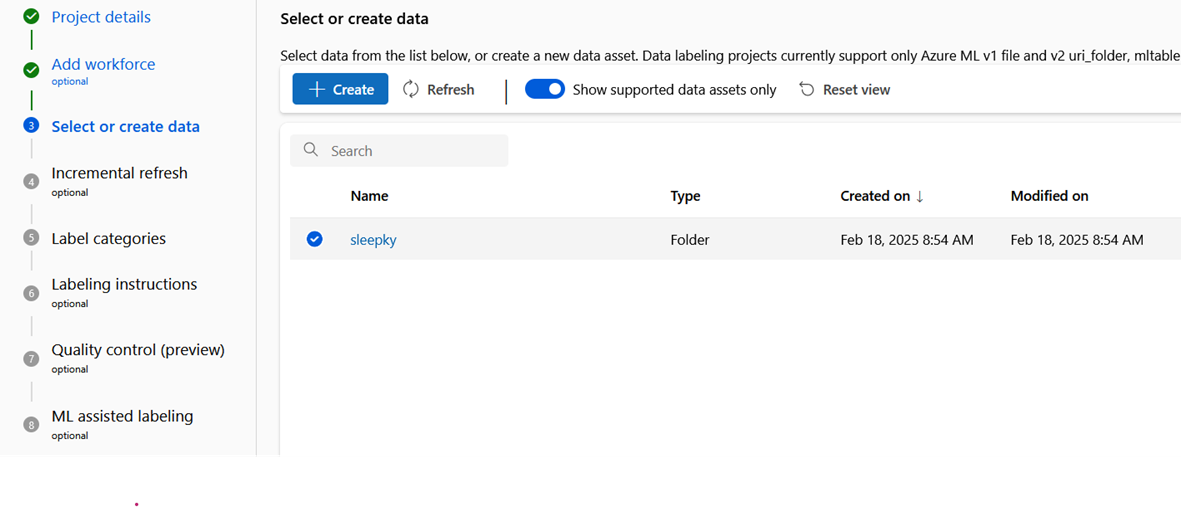
\includegraphics[width=\textwidth]{img/dataset_selection}
    \caption{Tvorba datasetu v AML}
    \label{fig:dataset_selection}
\end{figure}

V dalším kroku jsem nadefinoval kategorie, které budu chtít v obraze identifikovat.
V mém případě jsem zvolil label „slepice“.
Definice kategorií je na obrázku~\ref{fig:category_definition}.

\begin{figure}[h]
    \centering
    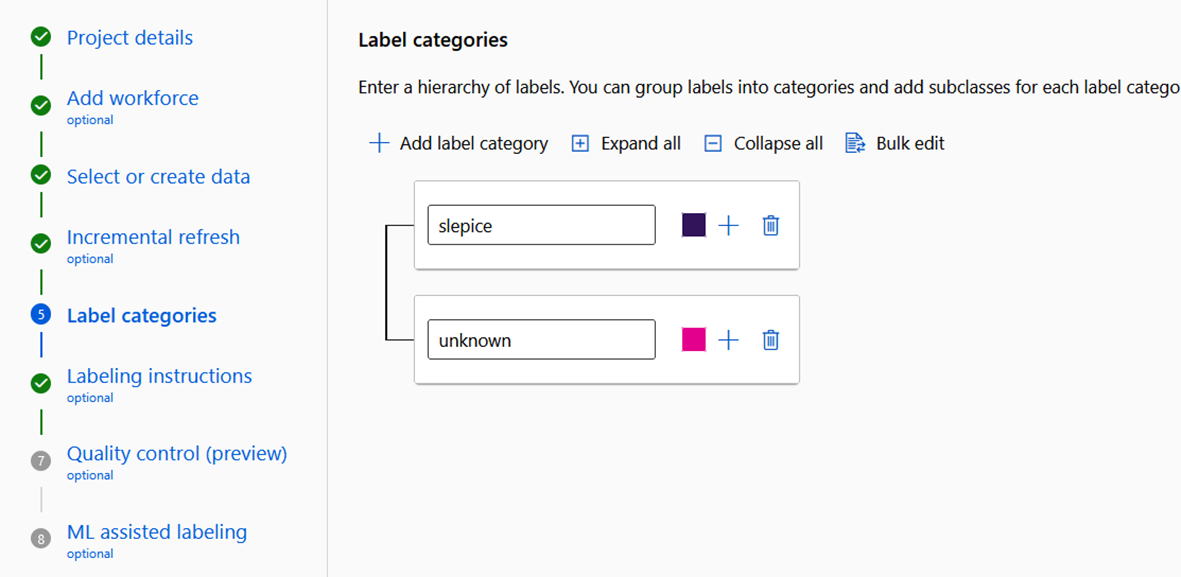
\includegraphics[width=\textwidth]{img/category_definition}
    \caption{Definice kategorií pro učení v AML}
    \label{fig:category_definition}
\end{figure}

V následujícím kroku následovala nejméně zábavná činnost.
Bylo třeba projít jednotlivé snímky a ručně vybrat oblasti, kde já jako člověk vidím slepici.
Oblast, kterou jsem označil se pak následně ukládá jako metadata k obrázku.
Tento proces je znárorněn na obrázku~\ref{fig:chicken_labeling}.

\begin{figure}[h]
    \centering
    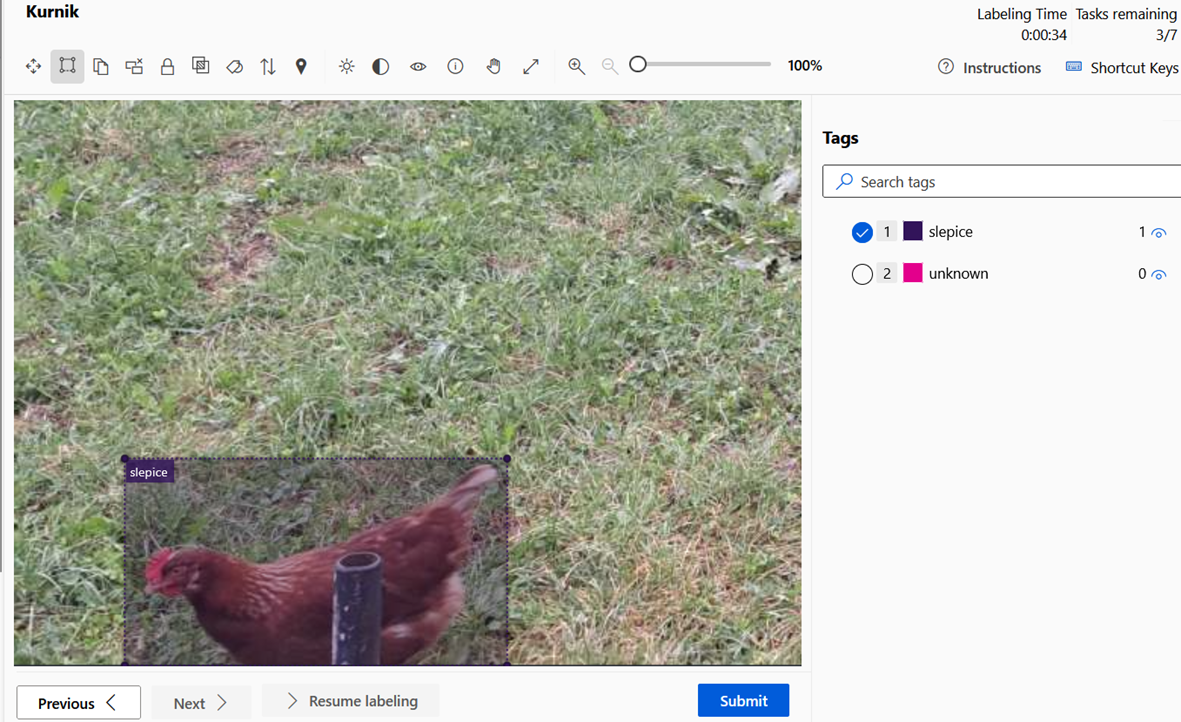
\includegraphics[width=\textwidth]{img/chicken_labeling}
    \caption{Označování slepic pomocí AML}
    \label{fig:chicken_labeling}
\end{figure}

Když se podařilo projít celý obrázkový dataset, mohl jsem vyexportovat „labeling“ data.
Jak jsem psal výše, mít kvalitní učící dataset je důležité, proto jsem exportoval pouze data, která se podařilo úspěšně označit.
Do fotogalerie se mi dostalo i několik nejasných snímků, případně těch, kde slepice nebyla vůbec.
Takové snímky jsem vyřadil.
Anotace jsem exportoval ve formátu COCO => dat odkaz do slovniku
Formát COCO (Common Objects in Context) je standardní formát pro anotaci obrázků používaný ve strojovém učení a počítačovém vidění.
Jeho hlavním cílem je poskytnout strukturu pro uložení informací o objektech v obrázcích, což umožňuje efektivní trénink a hodnocení modelů detekce objektů, segmentace a dalších úloh počítačového vidění.
Obrázek~\ref{fig:create_learning_project} ukazuje jak například může vypadat nastavení pro export COCO formátu z AML.

\begin{figure}[h]
    \centering
    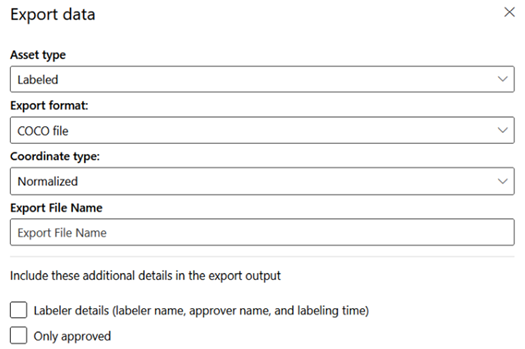
\includegraphics[width=\textwidth]{img/export_coco_format}
    \caption{Export metadat k obrázkům z AML do COCO formátu}
    \label{fig:export_coco_format}
\end{figure}

Soubor obsahuje několik klíčových sekcí: images, annotations, a categories.\newline
Zde je popis jednotlivých částí daného JSON souboru ve formátu COCO:
\begin{enumerate}
    \item images: Tato sekce obsahuje informace o každém obrázku v datasetu.
    \begin{itemize}
        \item id: Unikátní identifikátor obrázku (zde 1).
        \item width a height: Rozměry obrázku (zde 534 pixelů x 291 pixelů).
        \item file\_name: Cesta k souboru obrázku včetně názvu souboru.
        \item coco\_url, absolute\_url: Adresy, kde je obrázek uložen, ať už v cloudovém sandboxu (coco\_url) nebo přes URL pro přímý přístup (absolute\_url).
        \item date\_captured: Čas a datum zachycení obrázku v UTC formátu.
    \end{itemize}
    \item annotations: Tato sekce popisuje anotace neboli poznámky k jednotlivým objektům na obrázcích.
    \begin{itemize}
        \item id: Unikátní identifikátor anotace (zde 1).
        \item category\_id: Odkazuje na kategorii objektu (zde 1, což odpovídá \"slepice\").
        \item image\_id: ID obrázku, na který se tato anotace vztahuje.
        \item area: Relativní plocha objektu na obrázku (zde 0.016).
        Tato hodnota je často normalizována vzhledem k velikosti obrázku.
        \item bbox: Vektor čtyř čísel, který definuje obdélník (bounding box) okolo objektu na obrázku.
        Hodnoty jsou obvykle normalizované, takže se pohybují mezi 0 a 1 a odpovídají relativním souřadnicím a rozměrům (x, y, šířka, výška).
    \end{itemize}
    \item categories: Tato sekce obsahuje seznam kategorií, do kterých mohou objekty na obrázcích patřit.
    \begin{itemize}
        \item id: Unikátní identifikátor kategorie.
        \item name: Jméno nebo popis kategorie (zde \"slepice\" a \"unknown\").
    \end{itemize}
\end{enumerate}

Tento JSON tedy popisuje dataset obsahující obrázek s jedním označeným objektem, který patří do kategorie \"slepice\".
COCO formát umožňuje uložení komplexních a strukturovaných dat o objektech na obrázcích, což je velmi užitečné pro trénování a testování modelů strojového učení.
Příklad tohoto formátu metadat pro strojové učení je na obrázku~\ref{fig:coco_format}.

\begin{figure}[h]
    \centering
    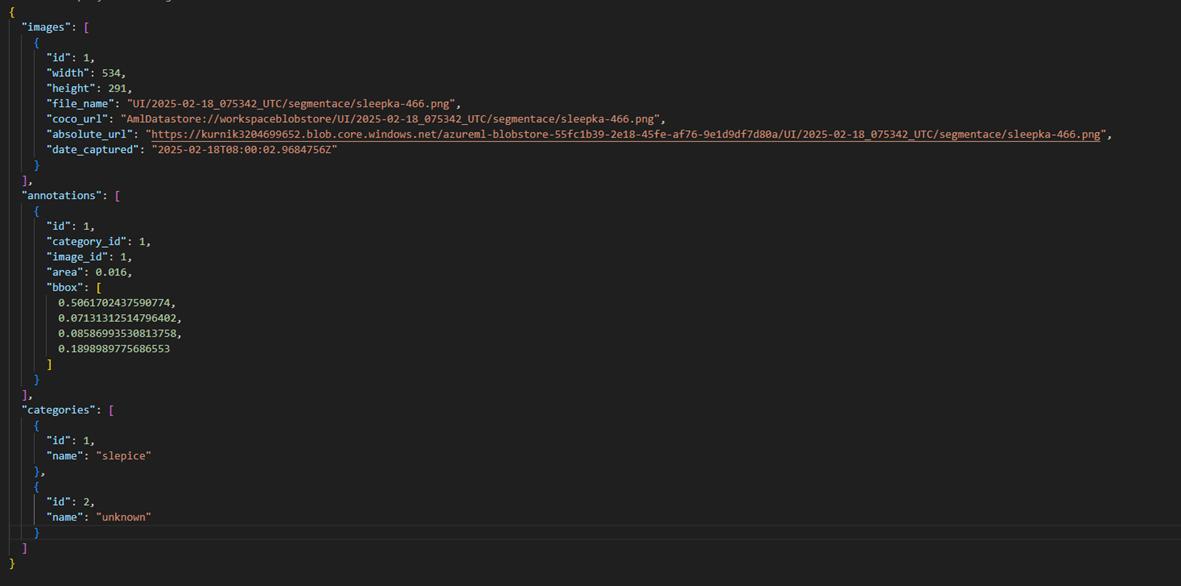
\includegraphics[width=\textwidth]{img/coco_format}
    \caption{Vytvoření nového projektu v AML}
    \label{fig:coco_format}
\end{figure}

\subsection{Doučování modelu Yolov11 o novou třídu}\label{subsec:doucovani-modelu-yolov11-o-novou-tridu}
V předchozí sekci jsem si popsali jak vytvořit zdroje dat a nyní jsme připraveni, vyučit existující model.
Doučovat doma existující model je relativně složité, ale díky výborné dokumentaci na strankach https://docs.ultralytics.com/ jsem to zvladnul.
Základem pro úspěšné a efektivní učení je hardware.
Hlavně GPU, protože trénování modelů hlubokého učení je výpočetně náročné.
Vypozoroval jsem, že největší vliv na učení má velikost paměti grafické karty.
V mém případě byla použita Nvidia RTX 4070.
O stavbě a následném učení neuronových sítí by se nechalo desítky stránek, ale to není předmětem mojí práce.
Rád bych alespon představil blokové schema učícího procesu.\newline
\newline
Pro učení jsem použil script, ktery jsem si pripravil.
Volání jednotlivých kroků pro učení je znázorněno na screenshotu učící metody na obrázku~\ref{fig:learn_script}

\begin{figure}[h]
    \centering
    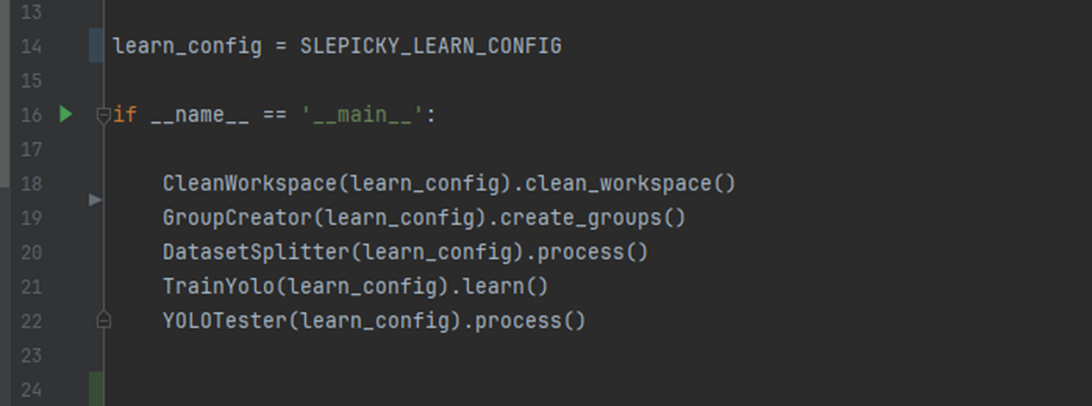
\includegraphics[width=\textwidth]{img/learn_script}
    \caption{Vytvoření nového projektu v AML}
    \label{fig:learn_script}
\end{figure}

\paragraph*{Krok 1 - CleanWorkspace}

Tento krok je zodpovědný za přípravu pracovního prostředí před zahájením tréninkového procesu.
Odstranuji v něm archivaci stávajících dat a modelů, které mi ve workspace zůstaly z předchozich běhů a již nejsou potřebné.
Čištění pomáhá zabránit kolizím s předchozími seancemi a udržet v něm pořádek, což zajišťuje, že nové modely a datové soubory jsou aktuální a správně organizované.

\paragraph*{Krok 2 - GroupCreator}

Tento krok se zaměřuje na organizaci dat do různých skupin pro trénování a testování modelu.
Data mám rozdělena v několika různých adresářích a tento krok má na starost jejich správné složení.
Stejná data používám výuků modelu na počítání slepic, detekce vetřelce a plánované reidentifikace slepic.

\paragraph*{Krok 3 - DatasetSplitter}

Proces rozdělení datasetu je klíčový pro oddělení trénovací, validační a testovací sady.
Rozdělení může být prováděno v daných poměrech, například 70% trénovací data, 15% validační data a 15% testovací data.
Správné rozdělení dat je důležité pro zajištění objektivního hodnocení modelu, aby se předešlo přeškolení.
Tento krok také zajišťuje, že žádné datové soubory nejsou opominuty a že rozdělení je náhodné a reprezentativní.

\paragraph*{Krok 4 - TrainYolo}

Jedná se o hlavní krok, kde je model YOLOv11 trénován na trénovacích datech.
Proces zahrnuje několik iterací (epoch) přes trénovací data, během kterých model aktualizuje své váhy podle chybného odhadu.
Na obrázku~\ref{fig:train_yolo}.


\begin{figure}[h]
    \centering
    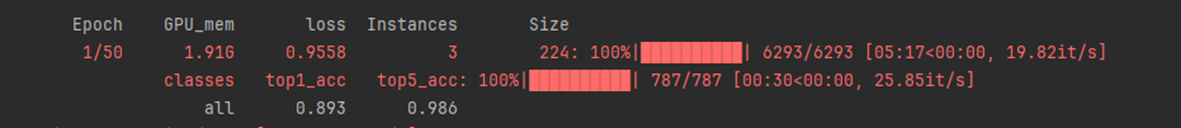
\includegraphics[width=\textwidth]{img/train_yolo}
    \caption{Proces trénování YOLOv11 modelu}
    \label{fig:train_yolo}
\end{figure}

Během trénování se sleduje výkonnost modelu na validačních datech, která zabraňují přeškolení.
Přeškolení si můžeme představit například u modelu, který rozpoznává kačeny, kočky a slepice.
I když všechny konfigurační parametry byly správně,  systém v některých případech špatně identifikoval kočku.
Až zpětnou analýzou trénovacích dat bylo zjištěno, že došlo k přeškolení.
System identifikoval kachnu nikoliv podle tvaru jejího těla, případně zabarvení, jako to udělá člověk, ale podle toho, zda na obrázku byla ci nebyla tráva.
To pak vedlo k tomu, že pokud byla kočka na trávě, byla označena za kachnu.
Spusti trénovací smyčku je jednoduché.
Bylo třeba předat jen několik základních parametrů.
\newline
Training Parameters\newline
Epochs: 50\newline
Batch Size: 16\newline
Pretrained: True (using pretrained weights)\newline
Data Path: c:/kurnik/klasifikace/kurnik\_learn\_temp/train\newline

50 Epoch známená kolik poběží učících cyklů.\newline
Batch Size – specifikuje kolik vláken poběží paralelně, je třeba dbát na velikost pameti grafické karty\newline
Pretrained – říká, že budeme rozšiřovat již naučený model\newline
Data Path – specifikuje odkud se mají vzit data k učeni.\newline

\paragraph*{Krok 5 - YOLOTester:}

Po úspěšném tréninku modelu je nutné jeho testování na dříve oddělené testovací sadě.
Tento krok zahrnuje vyhodnocení výkonnosti modelu pomocí metrik, jako je přesnost, citlivost.
Testování nám poskytuje objektivní zpětnou vazbu o tom, co za objekty model umí ve snímcích rozpoznat. Důležíté je předkladat pro testování snímky, které během tréninku neviděl.
Na základě testovacích výsledků jsem pak následně prováděl úpravy učicích parametrů, případně jsem dodával další data do učícího datasetu.

\begin{figure}[h]
    \centering
    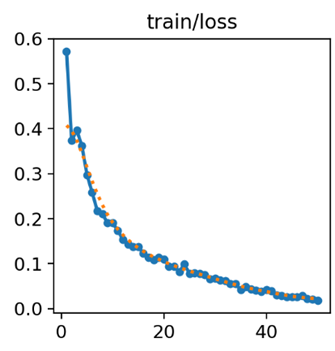
\includegraphics[width=\textwidth]{img/loss_funkce}
    \caption{Graf loss funkce v závyslosti na počtu etap}
    \label{fig:loss_funkce}
\end{figure}

Graf který je automaticky generováný při učení nám umožnuje sledovat, jak dobře se model učí vzhledem k časové ose tréninku.
Tento graf typicky zobrazuje ztrátovou funkci (loss) na svislé ose (Y) a počet trénovacích epoch nebo kroků na vodorovné ose (X).

\begin{figure}[h]
    \centering
    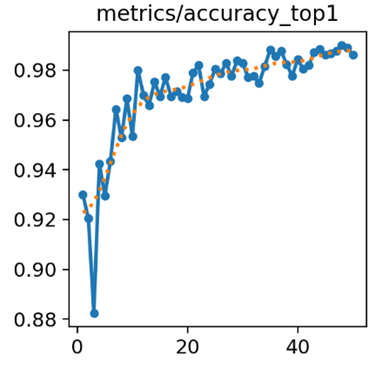
\includegraphics[width=\textwidth]{img/top1_accuracy}
    \caption{Vytvoření nového projektu v AML}
    \label{fig:top1_accuracy}
\end{figure}

Tento graf se zaměřuje na metriku přesnosti, konkrétně na \"top-1 accuracy,\" která měří, jak často je nejpravděpodobnější (nejvyšší hodnocená) předpověď modelu správná.

Výsledky detekce jsou demostrovány na obrázcích~\ref{fig:chicken_detection1},~\ref{fig:chicken_detection2},~\ref{fig:chicken_detection3},~\ref{fig:chicken_detection4},

\begin{figure}[h]
    \centering

    \begin{subfigure}[t]{1\textwidth}
        \centering
        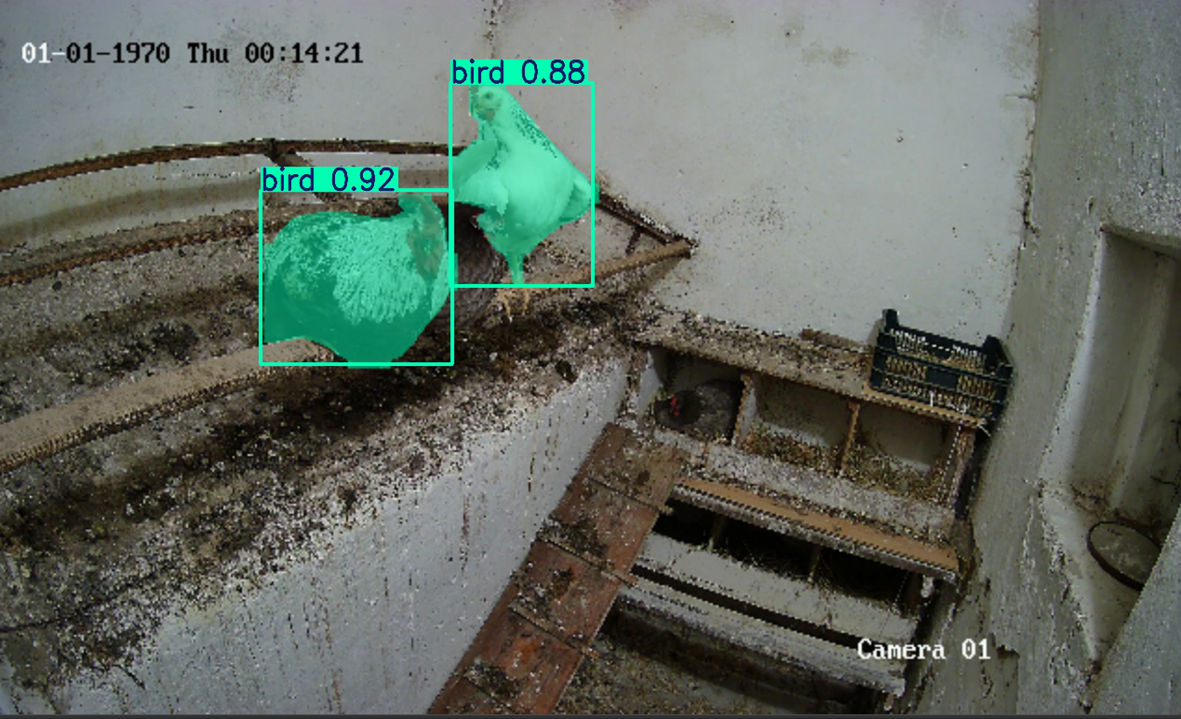
\includegraphics[width=\textwidth]{img/chicken_detection1}
        \caption{Výsledek detekce slepic}
        \label{fig:chicken_detection1}
    \end{subfigure}

    \begin{subfigure}[t]{1\textwidth}
        \centering
        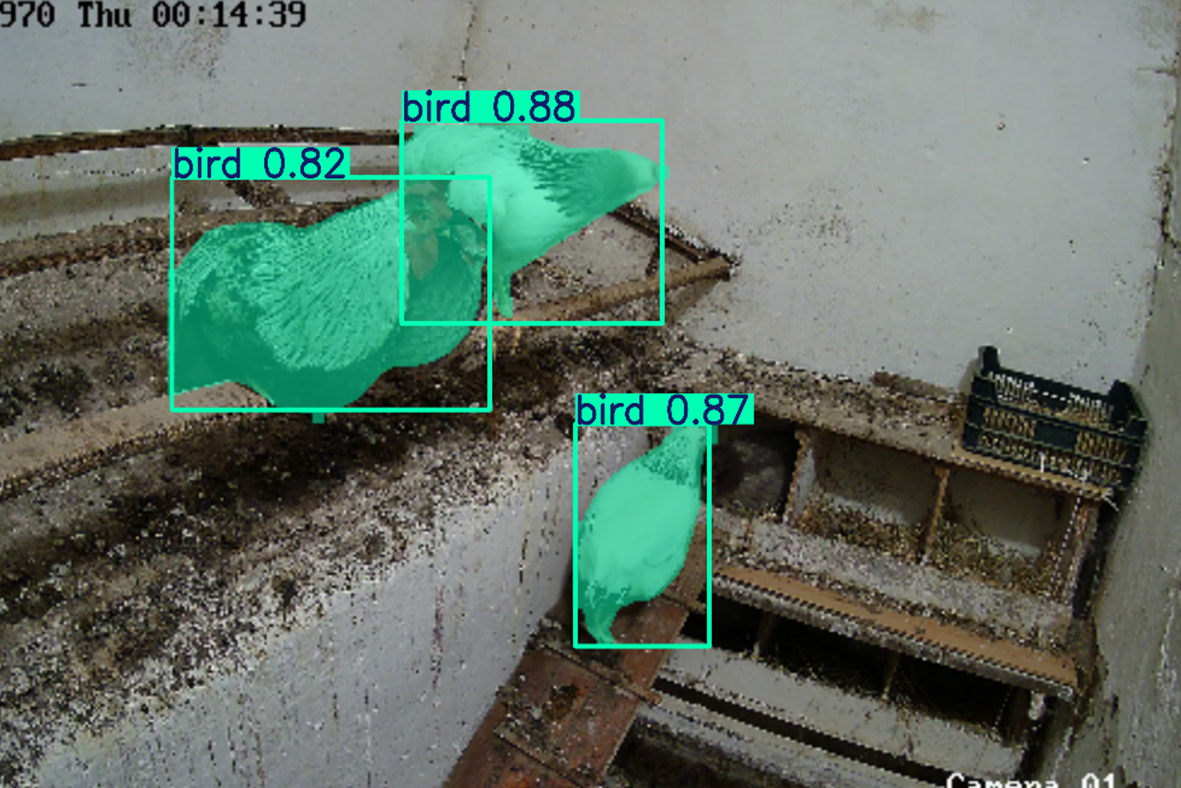
\includegraphics[width=\textwidth]{img/chicken_detection2}
        \caption{Výsledek detekce slepic}
        \label{fig:chicken_detection2}
    \end{subfigure}

    \begin{subfigure}[t]{1\textwidth}
        \centering
        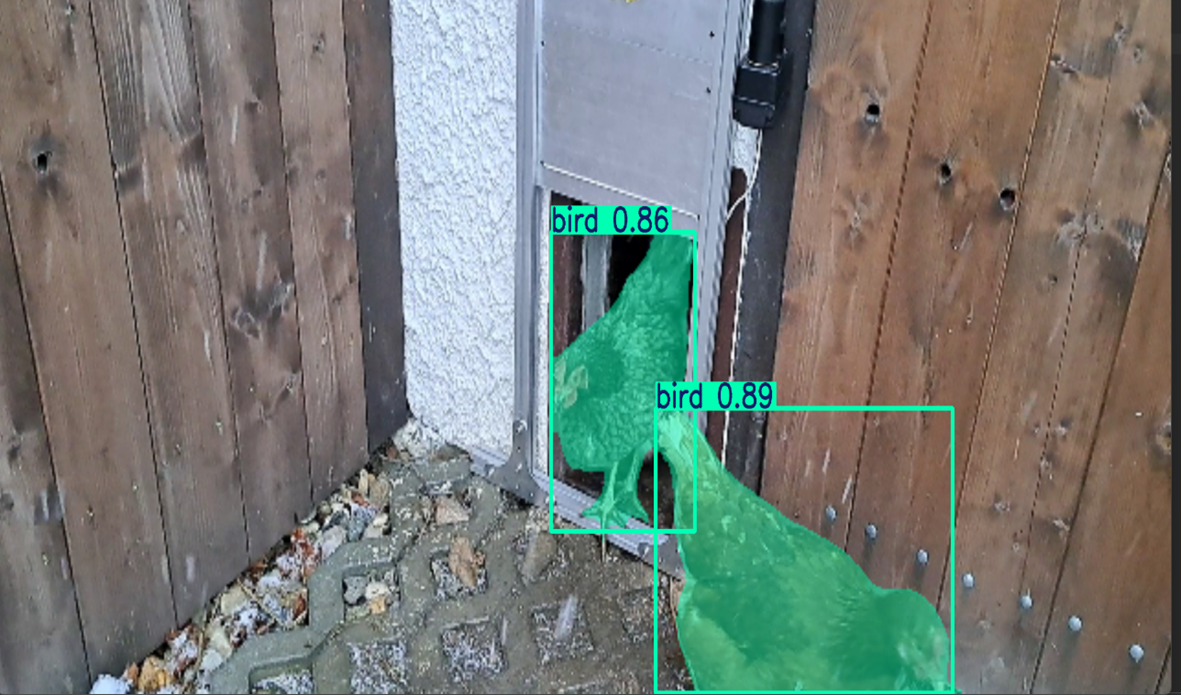
\includegraphics[width=\textwidth]{img/chicken_detection3}
        \caption{Výsledek detekce slepic}
        \label{fig:chicken_detection3}
    \end{subfigure}

    \begin{subfigure}[t]{1\textwidth}
        \centering
        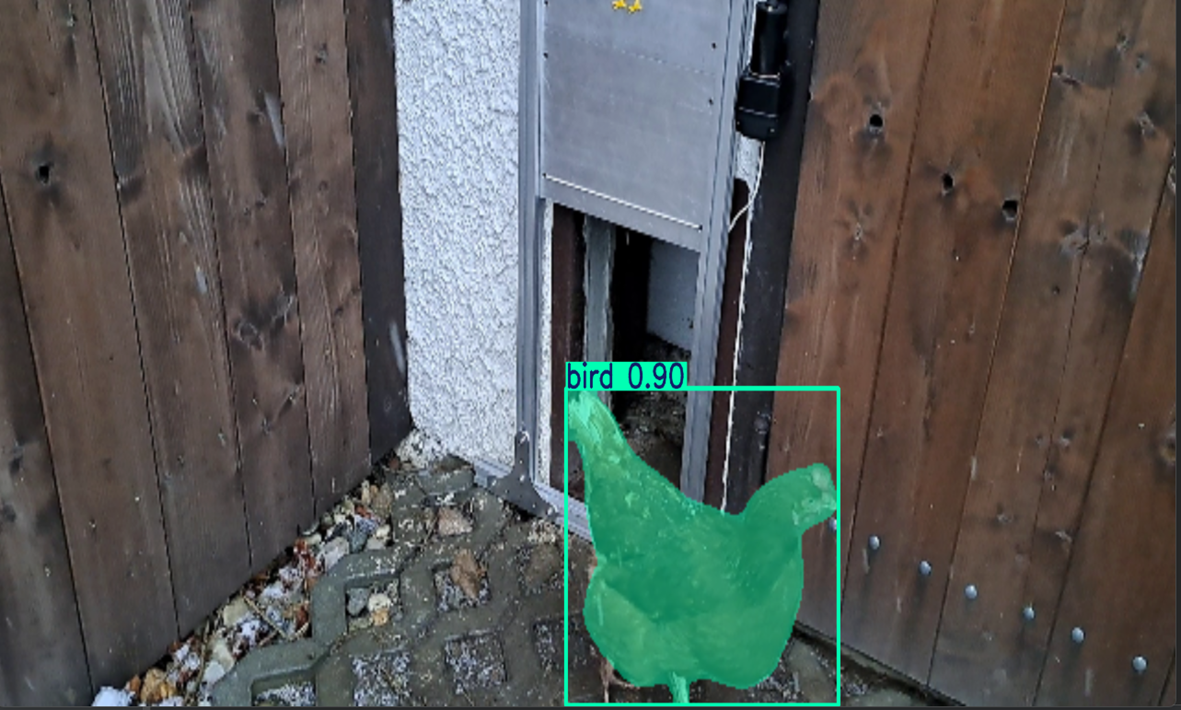
\includegraphics[width=\textwidth]{img/chicken_detection4}
        \caption{Výsledek detekce slepic}
        \label{fig:chicken_detection4}
    \end{subfigure}
\end{figure}

%todo fix render obrázků
\newpage
\section{Segmentace objektů pomocí strojového učení}\label{sec:klasifikace-a-segmentace-objektu-pomoci-strojoveho-uceni}

Image segmentation je technika v počítačovém vidění, která má za cíl rozdělit obrázek na několik segmentů nebo oblastí pro jednodušší analýzu.
Cílem image segmentation je identifikovat a rozlišit různé objekty nebo části obrázku, což může být užitečné pro různé aplikace, jako je rozpoznávání objektů, detekce hranic, klasifikace a další analytické úlohy.
V mém případě jsem chtěl využít tuto techniku k tomu, abych identifikoval, která slepice snesla vajíčko, abych tak získal statistiku o tom v jaké kondici slepice jsou a jak dobře snáší.
Existuje několik možností, jak slepici identifikovat, já jsem se rozhodl pro rozpoznání slepice z obrazu.

Nejdříve jsem začal pracovat na získání a přípravě dat.
Shromáždil jsem dataset snímků slepic z kurníku, který pokrývá různé úhly pohledu, osvětlení a pozice.
Dataset jsem anotoval.
V tomto případě byla tvorba anotačního souboru významně složitější, protože bylo třeba nejenom identifikovat, že slepice je na obraze, ale identifikovat její konkrérní tvar, případně jenom část těla.
Znamenalo to tedy ručně projít jednotlivé snímky a myší vyklikat potřebné oblasti, což je znázorněno na obrázku~\ref{fig:label_segmentation}.

\begin{figure}[h]
    \centering
    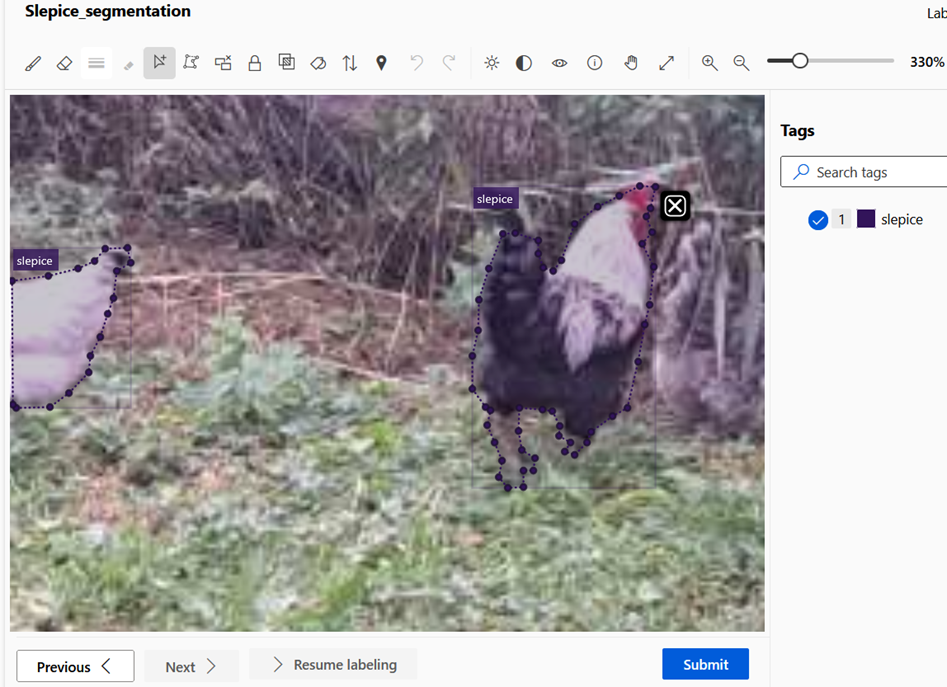
\includegraphics[width=0.8\textwidth]{img/label_segmentation}
    \caption{Proces tvorby metadat pro trénofání segmentace}
    \label{fig:label_segmentation}
\end{figure}

1.	Obecná zásada říká, že platí přímá úměra mezi množstvím trénovacích dat a kvalitou modelu.
Toto jsem mohl vyřešit větším počtem obrázku v testovacím datasetu nebo použít techniku augmentace dat.
To je postup, který jsem zvolil já. Na obrázky jsem aplikoval řadu transformací, které přispěly k různorodosti dat.\newline
\newline
Rotace - otáčení obrázků o náhodně vybrané úhly, aby se model stal invariantním vůči natočení objektů.\newline
Škálování - změny velikosti obrázků buď zmenšením nebo zvětšením, aniž by se změnil poměr stran, což pomáhá modelu lépe zvládat objekty různých velikostí.\newline
Oříznutí (cropping) - vyříznutí náhodných částí obrázku. \newline
To pomáhá modelu naučit se, že objekty mohou být částečně oříznuty.\newline
Překlopení (flipping) - horizontální nebo vertikální zrcadlení obrázku pro zvýšení variability dat.\newline
Změna jasu, kontrastu a saturace - úprava těchto parametrů dělá model odolnějším vůči různým světelným podmínkám.\newline
Přidání šumu - přidání náhodného šumu do obrázků může pomoci modelu být méně citlivý na zašumění v datech.\newline
Posun (translation) - posunutí obrázku ve vodorovném nebo svislém směru, které pomáhá modelu rozpoznávat objekty při různých umístěních.\newline
Random Erasing - náhodné vymazání malých částí obrázku, které může pomoci vylepšit model proti částečnému zakrývání objektů.\newline
MixUp - směšování dvou obrázků a jejich odpovídajících anotací ke generování nových tréninkových vzorů.\newline
Mosaic Augmentation - kombinování čtyř různých obrázků do jednoho, což rozšiřuje kontext a zvyšuje variabilitu scén.\newline
\newline

Následovalo trénování segmentačního Modelu:
Řešení jsem postavil na YOLO11 z oficiálního repozitáře.
Díky knihovnám z projektu Ultralytics je volání přímočaré.
Na vstup jsem dal cestu k obrázkovému datasetu a anotačnímu souboru v COCO formátu.
Další parametry jsem pro výuku ponechal defaultní.
Počet epoch jsem ponechal na 50.
Již od 40 epochy model dosahoval přijatelné úrovně přesnosti při rozpoznávání a segmentaci slepic.

Výsledek segmentace je vidět na obrázku ~\ref{fig:segmented_chicks}.



\begin{figure}[htbp]
    \centering
    % První řádek
    \begin{minipage}[b]{0.8\textwidth}
        \centering
        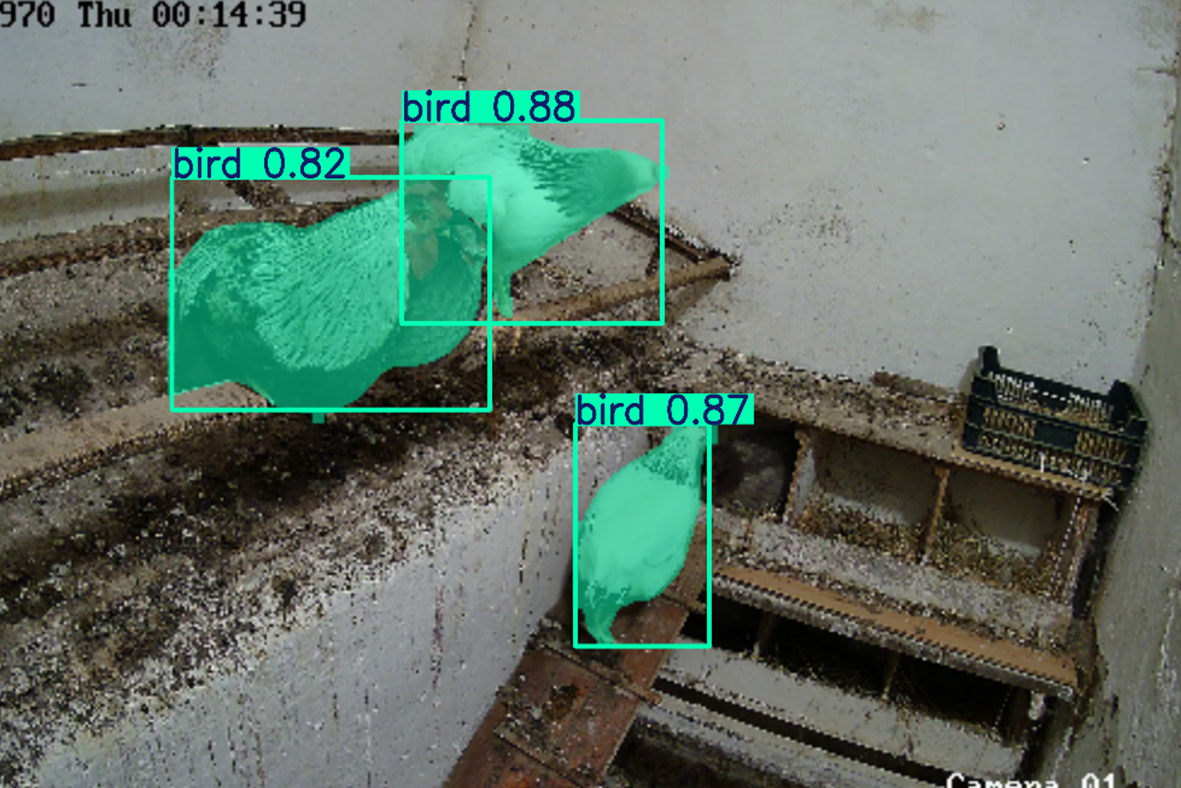
\includegraphics[width=0.8\textwidth]{img/chicken_detection2}
        \caption{Výsledek detekce slepic 1}
        \label{fig:chicken_detection2}
    \end{minipage}

    \vskip\baselineskip % Vertikální mezera mezi řádky

    % Druhý řádek
    \begin{minipage}[b]{0.8\textwidth}
        \centering
        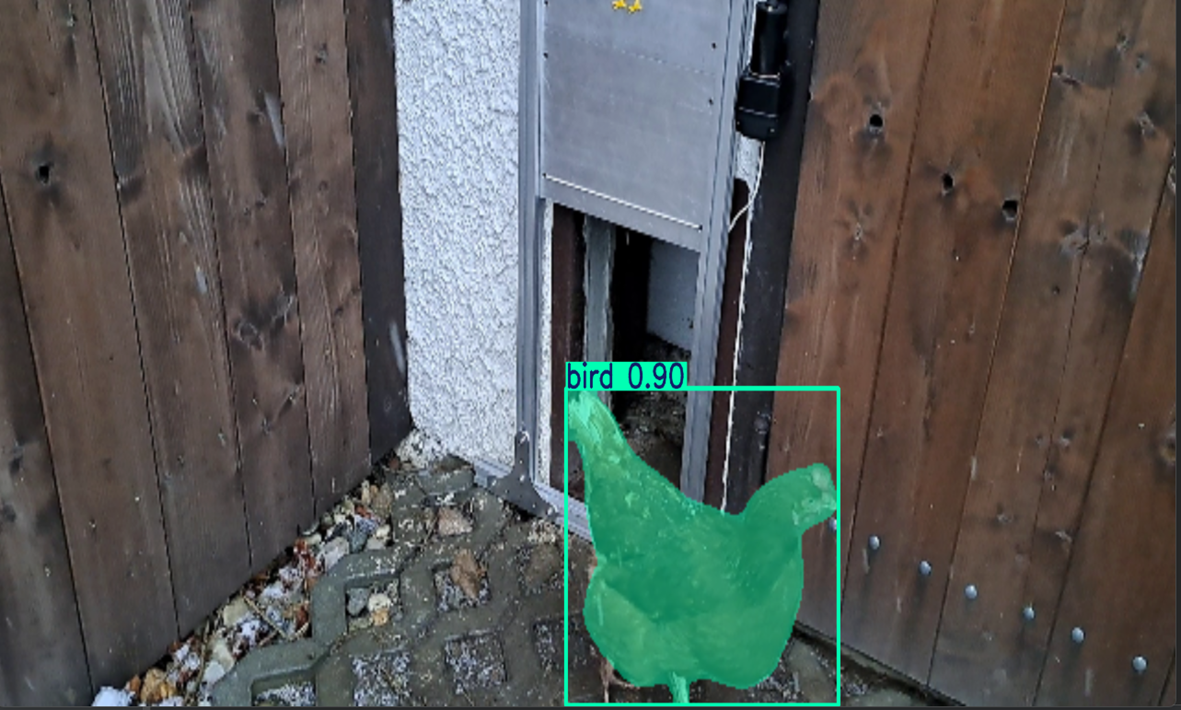
\includegraphics[width=0.8\textwidth]{img/chicken_detection4}
        \caption{Výsledek detekce slepic 2}
        \label{fig:chicken_detection4}
    \end{minipage}
\end{figure}



\newpage
\chapter{Nasazení systému do produkce}\label{ch:nasazeni-systemu-do-produkce}
\section{První pracovní zapojení a běh}\label{sec:prvni-pracovni-zapojeni-a-beh}
%- zjistilo se že bez poe je to špatná volba \newline
%- kamery žerou dost proudu\newline
%- bylo potřeba odladit nastavení kamer a jejich statické ip adresy, kamery měli zabezpečení na blokování ip address a tak\newline
%- byl problém s kontakty na váze takže se nakonec museli vyměnit lisované za pájené\newline
%- na stole to většinou funguje dobře \newline
Během prvního pracovního zapojení a spuštění systému se ukázalo několik klíčových aspektů, které je třeba optimalizovat pro zajištění spolehlivého provozu.
Jedním z prvních zjištění bylo, že absence technologie Power over Ethernet (PoE) není ideální, zejména proto, že kamery spotřebovávají značné množství elektrického proudu.
To vedlo k potřebě přehodnotit napájecí řešení.
\newline
Kromě napájení bylo nezbytné doladit nastavení kamer, včetně přiřazení statických IP adres.
Některé kamery totiž disponovaly bezpečnostními opatřeními, která blokovala IP adresy, což způsobovalo komplikace v připojení a stabilitě systému.
\newline
Dalším technickým problémem byly kontakty na váze, kde se původně používaly lisované spoje, které se ukázaly být nespolehlivými.
Pro zajištění lepšího výkonu a spolehlivosti byly tyto spoje nahrazeny pájenými, což přineslo lepší výsledky.
\newline
Navzdory těmto problémům systém fungoval relativně dobře při testování na pracovním stole, což naznačuje, že se na této úrovni setkáváme s minimálními problémy.
Tyto zjištění poskytují pevný základ pro další optimalizaci a nasazení systému v reálných podmínkách.


\newpage


\section{Nasazení do kurníku}\label{sec:nasazeni-do-kurniku}
%- bylo potřeba natahat elektřinu a internet \newline
%- elektřina nebyla problém vzala se z kůlny zkrz díru ve zdi\newline
%- horší to bylo s netem protože wifi signál do kurníku nedosáhne\newline
%- vyřešilo se to wifi extenderem od tplinku který má zárověň i ethernet výstup díky čemuž nemuselisme dlouhého tahati kabelu a šlo nám to vzduhem přes dvůr a ve stodole pak drátem\newline
%- kamery bylo potřeba napájet a taky připojit přes internet; zprvu jsem si myslel že poe nebude potřeba ale taha 230 by bylo zbytečné námahy takže jsem pořídil poe switch od tplinku a ten připojuje kamery\newline
%- bylo někde potřeba udělat místo kam se nainstaluje celá technologie kurníku\newline
%- zvolila se plechová bedna ze starého domovního rozvaděče do níž se pro jednotlivé prvky vytvožili na míru držáčky a pouzdra ps.: fotky z tisku a pak z rozvaděče\newline
%- jak se zrealizovala váha\newline
%- jak vypadá řídící jednotka pri room assistanta\newline
%- jaké tam jsou dveře pro slepice\newline
%- celé je to propojené s rpi 5 které to v kurníku řídí a s ním pak komunikuje nuc pomocí tail scailu ale to zas v další kapitole\newline
%- bylo potřeba zkalibrovat hmotnosti slepic a vajec

Nasazení systému Coopmaster přímo do kurníku vyžadovalo několik klíčových kroků, abychom zajistili jeho plnou funkčnost a efektivitu.
Jedním z prvních úkolů bylo natažení elektřiny a připojení k internetu.
Elektřina byla přivedena bez větších problémů; využili jsme stávající zdroje z kůlny prostřednictvím otvoru ve zdi.
\newline
Výrazně náročnější bylo zajistit internetové připojení, protože signál Wi-Fi nedosahoval až ke kurníku.
Toto jsme vyřešili instalací Wi-Fi extenderu od TP-Link, který nabízí také ethernetový výstup.
Toto řešení nám umožnilo přenášet data vzduchem přes dvůr, a dále pak ve stodole drátem, čímž jsme se vyhnuli nepotřebnému natahování kabeláže.
\newline
Dalším úkolem bylo napájení a připojení kamer přes internet.
Zpočátku jsem předpokládal, že Power over Ethernet (PoE) nebude nutné, ale poté, co by tahání 230V kabelů znamenalo nadměrné úsilí, jsem pořídil PoE switch od TP-Link, který tyto kamery napájí i připojuje.
\newline
Dále bylo nutné vytvořit prostor, kam nainstalovat veškerou technologii kurníku.
Pro tento účel jsme zvolili plechovou bednu ze starého domovního rozvaděče.
Do této bedny byly přesně vyrobeny držáčky a pouzdra pro jednotlivé komponenty, jak dokládají fotografie z výroby a samotného rozvaděče.
\newline
Při instalaci bylo důležité řešit i váhu systému a její kalibraci pro přesné měření hmotnosti slepic a vajec.
Řídící jednotka pro Home Assistant je součástí tohoto systému a zajišťuje bezproblémový provoz.
Dveře pro slepice jsou integrovány do celkového řešení a celé řízení probíhá prostřednictvím Raspberry Pi 5, které komunikuje s NUC pomocí řešení Tailscale, ale tuto problematiku rozvedeme v další kapitole.
\newline
Tento komplexní proces nasazení do kurníku neustále vyžadoval přesné plánování a realizaci, abychom zajistili vysokou úroveň automatizace a efektivity potřebnou pro moderní chov slepic.

\newpage


\section{Konfigurace vzdáleného přístupu}\label{sec:konfigurace-vzdaleneho-pristupu}
%- rpi propojene s nuckem a dev kompama přes tailscail\newline
%- v docker compose na nuckoj se vyrobila nová network jenom pro home assistanta a jeho propagaci na venek\newline
%- do vzniklé sítě se přidal ještě kontejner Cloudflared který zajišťuje tunel ven na cloudflare a přes jeho firewall a proxyny do internetu\newline
%- cloudflare tunel bylo potřeba namapovat na doménu kterou vlastníme\newline
%- pronajmul jsem si doménu u doméhového registrátora forpsi\newline
%- zmínění jaká plynou nebezpečí z tohoto řešení

Konfigurace vzdáleného přístupu k systému Coopmaster byla založena na robustní infrastruktuře, která zajišťuje bezpečné a efektivní propojení mezi klíčovými komponentami.
Raspberry Pi (rpi) bylo propojeno s NUC a vývojářskými počítači prostřednictvím Tailscale, což umožňuje vytvoření privátní sítě VPN, která je snadno spravovatelná a zajišťuje bezpečné spojení.
\newline
Pro Home Assistant byl na NUC v systému Docker vytvořen specifický síťový most.
Tento most je dedikovaný pouze pro Home Assistant a jeho potřeby komunikace s vnějším světem.
K této síti byl přidán i kontejner Cloudflared, který umožňuje vytvoření bezpečného tunelu na platformu Cloudflare.
Cloudflared zajišťuje průchod dat skrz Cloudflare firewall a proxy servery na internet, čímž zvyšuje bezpečnost a spolehlivost komunikace.
\newline
Aby byl tunel funkční, bylo nutné jej namapovat na naši vlastněnou doménu.
Pro tento účel jsem si registroval doménu u doménového registrátora Forpsi, což nám poskytlo potřebné DNS záznamy k propojení s Cloudflare.
\newline
Je důležité poznamenat, že taková konfigurace s sebou nese i jistá bezpečnostní rizika.
Primárním rizikem je možnost neautorizovaného přístupu, pokud není správně nakonfigurováno zabezpečení tunelu a neprovádí se pravidelné audity.
Dále mohou existovat zranitelnosti v softwaru kontejneru nebo sítě, které by mohly být zneužity, pokud nejsou průběžně aktualizovány.
Z těchto důvodů je klíčové udržovat systém aktualizovaný a implementovat vhodná bezpečnostní opatření.

\newpage

%\section*{---poznámky TODO ke smazání---}\label{sec:---poznamky-todo-ke-smazani---}
%- budeme potřebovat váhu pro kontrolu hnízd zda tam slepice je a nebo kolik je tam vajec\newline
%- budeme potřebovat ideálně ip kamery s vhodným IP krytím abychom mohly monitorovat kurník vevnitř a venku\newline
%- budeme potřebovat ovladačku asi arduino pro dveře, světlo, senzory teploty a vlhkosti\newline
%- předchozí věci je potřeba dostat na síť takže nějaké rpi pro předávání komunikace a směrování\newline
%- a všechno to musí řídit něco s dostatečným výkonem pro klasifikace třeba my tu máme nucka s RTX2080\newline
%- uživatelské rozhraní se rozhodlo že je zbytečné vyrábět vlastní a ztrácet tím čas lepší bude použít HA který disponuje všemi funkcemi je open source a má komunitu která ho udržuje
%- první řešení ale bude na stole takže se nemusíme zaobírat detaily kontkrétní instalace, alespoň pro zatím
%- implementace probíhala v jazyce python za využítí vypsaných knihoven viz readmečka modulů\newline
%- jak se konfiguroval logger, flask blueprinty, jak propojit python a arduino, jak na to s cronem/schedulerem, jak posílat mqtt a přijímat(jaká je struktura našich topiců, jak se to pojmenovává)
%- verzuje se to na github
%- na githubu běží workflow které vytváří jednolivé docker image pro každý modul a uploaduje je na můj docker hub kvůli snadnému deployi a distribuci po internetu

\newpage
\chapter{Ekonomická stránka projektu}\label{ch:ekonomicka-stranka-projektu}
Projekt Coopmaster je rozhodně revoluční řešení v chovatelské branži.
Každopádně se rozhodně nehodí jeho využití jako odpověď na snížení ceny za provoz malých domácích chovů.
Hlavním důvodem je už samotná pořizovací cena komponent, která je u mého prototypového řešení okolo 20 ticíc korun.
Je tedy rozhodně zbytečné instalovat systém do malého domácího kurníku, když samotná pořizovací cena předčí cenu vajec vyprodukovaných za 3 roky a to se ještě nebavím o licencích za software a energie potřebně pro běh systému.\newline
Potenciál tohoto nápadu by se dle mého dal určitě zúročit ve větších podnicích, kde bude možno naplno využít schopností celého řešení.
Například počítání by určitě pomohlo například na pastvách s ovcemi či kravami, kde jsou počty výrazně větší a je již složité a časově náročné ručně spočítat všechny kusy.
Dále by se potenciál kamer a neuronových sítí dal využít k detekci nemocných nebo zraněných zvířat.
Toto jsou faktory, které by rozhodně stálo za to vyzkoušet zlepšit.
Například pokud by systém správně s předstihem detekoval nějakou nemoc na jednom jedinci ve stádě krav, mohlo by to pomoci dříve zareagovat a zachránit zbytek stáda před uhynutím.
V takovém případě by se právě systém velice vyplatil, protože by vlastně zachránil firmu před krachem.\newline
Dále je určitě vhodné zmínit možnost automatizace krmení a čištění sídel zvířat.
To je věc, která se dá plně automatizovat a ušetřit tak čas a případně i pracovní sílu, která by jinak tyto činnosti konala.\newline
Na závěr tedy můžeme říct, že myšlenka tohoto systému se nevyplatí pro malé chovatele, pokud to nejsou techničtí nadšenci jako já.
Své uplatnění, ale najde u větších firem, který může v daných situacích i zachránit byznys.







\newpage
\chapter{Rozvržení práce do budoucna}\label{ch:rozvrzeni-prace-do-budoucna}
V tomto projektu vidím potenciál jak z osobního, tak i profesního hlediska.

Z osobního pohledu mě motivuje příležitost k sebevzdělávání, protože mě zajímá kompletní vedení projektu od počáteční myšlenky až k jeho realizaci.
Rád bych se aktivně zapojil do všech fází – od návrhu přes vývoj po řešení různých problémů.

Z profesního hlediska mě přitahuje vývoj těchto technologií, protože věřím, že v budoucnu budou mít klíčový význam.
To by mohlo zvýšit atraktivitu tohoto projektu, a časem by mohl přitáhnout pozornost investorů.
Například by jej mohl chtít financovat některý zemědělec, pod  podmínkou vývoje, implementace a podpory na jeho farmě, což by mi přineslo mnoho cenných zkušeností.

Na základě těchto úvah plánuji v projektu pokračovat a dále jej rozvíjet.
Níže uvádím funkcionality, které mám v úmyslu implementovat po dokončení této práce.\newline

\section{Koncept identifikace nejlepší nosnice}\label{sec:koncept-identifikace-nejlepsi-nosnice}

Při chovu slepic by bylo velmi užitečné vědět, kolik vajec která slepice snáší, protože to umožňuje farmáři sledovat produktivitu jednotlivých slepic.
Díky tomu může:
\begin{itemize}
    \item Optimalizovat chov: Identifikací slepic s vysokou a nízkou snáškou může farmář rozhodnout o selekci nebo o zvláštní péči pro méně produktivní slepice.
    \item Zlepšit zdraví slepic: Nízká snáška může být indikátorem zdravotních problémů. Včasná identifikace umožňuje podniknout kroky k léčbě nebo prevenci nemocí.
    \item Efektivněji plánovat krmení a zdroje: Sledování výkonu pomáhá v rozhodování o výživě a péči, aby byla maximalizována produkce vajec při optimálních nákladech.
    \item Zvýšit ziskovost: Monitorováním snášky lze zlepšit celkovou produktivitu farmy a tím i její ekonomickou efektivitu.
\end{itemize}

Celkově tedy znalost počtu vajec od každé slepice pomáhá v efektivním řízení chovu a zajišťuje lepší výsledky jak po stránce produkční, tak ekonomické.
Abych toho dosáhl, potřebuji být schopen jednotlivé slepice identifikovat a tuto informaci propojit s momentum, kdy slepice sense v kurniku vejce.
V sekci  pridat odkaz  “Vaha”, je popsan mechanismus, kdy pravidelnou analyzou casove rady, kterou poskytuje vaha ziskame informaci o casove udaji, kdy bylo vejce sneseno.
Pak jiz jen staci identifikovat, ktera z nasich slepic byla v tu dobu v hnízdě.
Existuje několik variant, jak slepice identifikovat, já jsem se rozhodl využít k identifikaci obrazovou analýzu.
Postupuji následujícím způsobem.
Nejprve procházím videozáznam a identifikuji oblasti, kde se slepice nacházejí.
Tyto oblasti následně vystřihnu a uložím do samostatných souborů.
Poté procházím tyto menší obrázky a pomocí segmentace vystřihnu plochu, kde je slepice, zatímco ostatní části zůstanou bílé.
Takto vyříznuté obrázky převádím na tenzory.
Převod na tenzor znamená, že dvourozměrný obraz (matice pixelů) převedu do vícerozměrné datové struktury, která dokáže reprezentovat různé vlastnosti obrazu a je vhodná pro strojové učení a další matematické zpracování.
Tímto způsobem získám numerickou reprezentaci obrazu, se kterou mohu efektivně pracovat.
Získané tenzory porovnávám se vzorovými vektory uloženými v databázi.
Pokud je vektor shodný, znamená to, že jsem našel odpovídající slepici, a podařilo se mi ji tak identifikovat.

Algoritmus tedy na počátku vezme jako vstup obrázek z kamery viz obrázek~\ref{fig:source_chick_image}.
Dále je obrázek segmentován a jsou vyjmuty pouze tvary, které algoritmus vyhodnotil jako slepice viz obrázek~\ref{fig:segmented_chicks2}.
Na závěr je pro každý výřez vypočítán tenzor na jehož základě jsou slepice roztřízeny do jednotlivých skupin podle barvy viz obrázek~\ref{fig:chicks_in_clusters}.



\begin{figure}[h]
    \centering
    \begin{subfigure}[t]{1\textwidth}
        \centering
        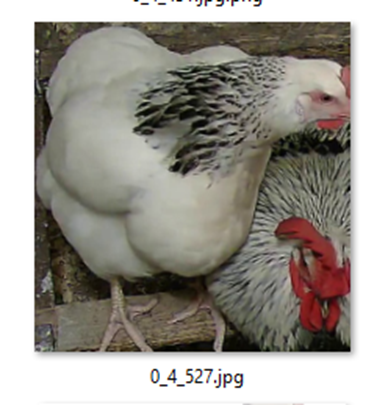
\includegraphics[width=\textwidth]{img/source_chick_image}
        \caption{Jeden ze vstupů do algoritmu pro nosnice}
        \label{fig:source_chick_image}
    \end{subfigure}

    \begin{subfigure}[t]{1\textwidth}
        \centering
        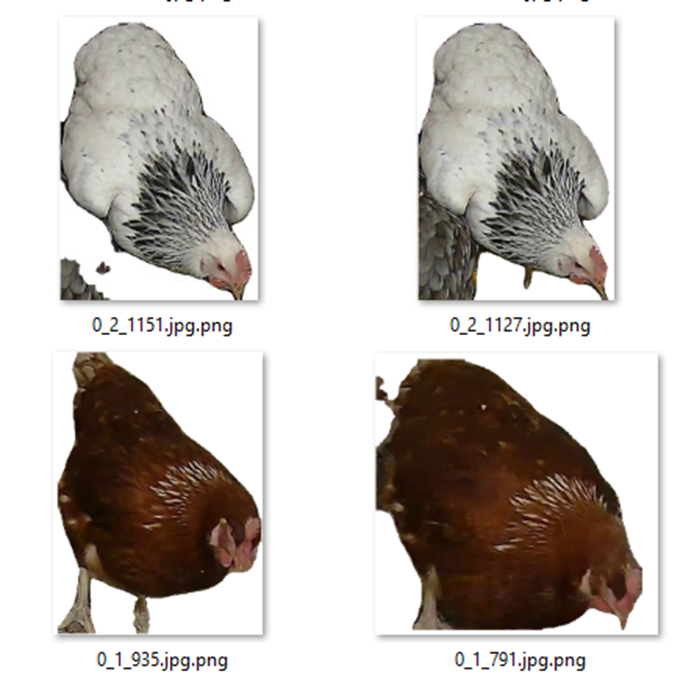
\includegraphics[width=\textwidth]{img/segmented_chicks}
        \caption{Segmentované slepice z fotek}
        \label{fig:segmented_chicks2}
    \end{subfigure}

    \begin{subfigure}[t]{1\textwidth}
        \centering
        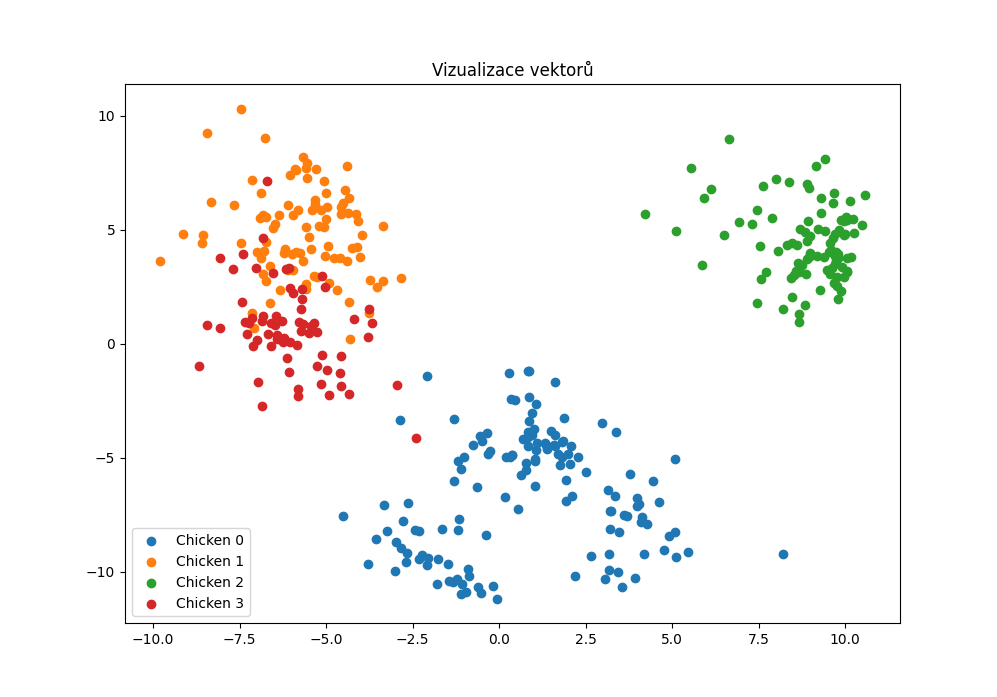
\includegraphics[width=\textwidth]{img/chicks_in_clusters}
        \caption{Algoritmem rozdělené slepice dle tenzorů}
        \label{fig:chicks_in_clusters}
    \end{subfigure}
\end{figure}

\section{Vylepšení konstrukce dvířek}\label{sec:vylepseni-konstrukce-dvirek}
Vylepšení konstrukce dvířek a realizace finálního řešení je jeden z plánů do budoucna pro tento projekt.
Jak již bylo zmíněno v popisu současné konstrukce v sekci~\ref{sec:konstrukce-dvirek}, aktuální konstrukce je příliš drahá na výrobu a také zbytečně robustní.
Pro finální instalaci v následujících větách popíšu návrh na realizaci produkční konstrukce.\newline
Konstrukce by měla být levnější na výrobu i na materiál a zároveň stejně bezpečná a výkonná jako ta stávající prototypová.
Nový rám bude tvořen z železných U profilů použitých zároveň jako vodící lišty pro posuv dvířek.
Posuvný plát bude z plastové desky.

\subsection*{Navíjecí mechanismus}\label{subsec:navijeci-mechanismus}
Způsob ovládání neboli napájení se nemění takže není třeba dělat žádné úpravy na řídící jednotce popsané detailněji v sekci~\ref{sec:ridici-jednotka}.
Pohyb bude dvířkům dodávat malý elektrický naviják vlastní konstrukce.
Díky vlastnímu návrhu bude možno celý rám navijáku navrhnout pomocí CAD programu a následně ho celý vyrobit na 3D tiskárně.
Tento způsob výroby šetří čas a je zajiště přiměřeně stejná kvalita u všech součástek.
Pohonnou jednotkou navijáku bude 12 V elektromotor model JGA25-370 na stejnosměrné napětí s vestavěnou převodovkou.
Díky převodovce dokáže motor vyvinout kroutící moment až 130N na 1cm dlouhé páce, což je na pohyb dvířek dostačující.
Vývodový hřídel z převodovky elektromotoru bude připevněn k navíjecímu bubnu o průměru okolo 15 mm.
Na navíjecím bubnu bude připevněno i lanko, které se bude používat na vytahování dvířek nahoru.
Pohyb dolů je zajištěn díky gravitaci, díky čemuž stačí povolit lanko a dvířka sama sjedou dolů.
Jako pokračování v ose otáčení motoru a bubnu bude k bubnu připevněn malý šnekový hřídel s maticí.
Matici je zamezeno otáčení opřením o rám navijáku takže se při otáčení hřídele se bude matice posouvat.
Tohoto pohybu bude využívat poslední součást navijáku a to systém dorazů, aby bylo možno nastavit maximální počet otáček bubnu a nedošlo tak k úplnému odvinutí lanka.
Úplné odvinutí lanka by v případě, že by se motor pořád točil, znamenalo, že se lanko zase začne navíjet opačným směrem, což obrátí navíjecí logiku navijáku.
Řídící jednotka totiž počítá pouze s jedním směrem otáčení a nepočítá s náhlým přehozením směru otáček motoru pro navíjení a odvíjení.


%konstrukce dveří - instalováno
%- zdroj 12V
%- rám z
%- naviják je s dvířky přopojen lankem
%- navíjecí systém / systém navijáku
%- 12V motor s převodovkou, rychlostí otáčení 60rpm
%- navíjecí buben vytištěný na 3d tiskárně
%- dorazový systém
\section{Vylepšení funkcionality služby Room Assistant}\label{sec:vylepseni-funkcionality-sluzby-room-assistant}

// TODO

- lze doimplementovat automatické ovládání světel a dvířek pro případ nefunkčnosti home assistanta
- resi rano otevirani dveri kurniku a vecer zavirani
- Integrace se sluzbou  - https://api.sunrise-sunset.org/json?lat=50\&lng=14.5
- dvere se nezavrou pokud nejsou slepice doma (kontrolu lze provézd zavoláním přímo na chicken watch guarda)
- dvere v modu automatickeho zavirani si volaji o data kdy zavirat https://kodim.cz/czechitas/daweb/js2/server-komunikace/cv-volani-api/vychod-zapad

\newpage
\chapter{Teoretické pojmy}\label{ch:teoreticke-pojmy}
\section*{Docker Engine}\label{sec:docker-engine}
Jedna z technologií používaných pro kontejnerizaci je Docker Engine~\cite{kontejnerizace-docker}.
Používá se pro tvorbu, správu, orchestraci, verzování a nasazování jednotlivých kontejnerů.

\section*{Docker Compose}\label{sec:docker-compose}
Docker compose~\cite{kontejnerizace-docker-compose} je nástroj pro Docker, který nám umožňuje tvořit komplikované ekosystémy jednotlivých kontejnerů, jež spolu v rámci něho mohou spolupracovat.
Pomáhá nám například se síťováním nebo konfigurací kontejnerů.


\section*{Mikroservisní architektura}\label{sec:microservice-architecture}
Mikroservisní architektura je přístup k vývoji softwarových aplikací, kdy je celek rozdělen na malé, nezávislé služby nazývané mikroservisy.
Každá služba běží samostatně, komunikuje s ostatními službami pomocí dobře definovaného API a je zaměřena na konkrétní funkcionalitu.
Tento model umožňuje snadnější údržbu, škálovatelnost a flexibilitu systému.


\section*{Jazyk Python}\label{sec:python}
Python je vysokoúrovňový programovací jazyk známý svou jednoduchou a čitelnou syntaxí.
Podporuje několik programovacích paradigmat, včetně objektově orientovaného, procedurálního a funkcionálního programování.
Python je široce používán v různých oblastech, jako je webový vývoj, vědecké výpočty, umělá inteligence, strojové učení a datová analýza.
Disponuje rozsáhlou standardní knihovnou a množstvím externích modulů, které usnadňují vývoj komplexních aplikací.
Je multiplatformní, což znamená, že programy v Pythonu lze spouštět na různých operačních systémech.


\section*{Wire}\label{sec:wiring}
Wiring je open-source programovací jazyk a vývojové prostředí určené pro práci s mikrokontroléry.
Jeho cílem je usnadnit programování elektronických zařízení a interaktivních projektů, zejména pro umělce, designéry a studenty.
Syntaxe jazyka Wire vychází z jazyka C++ a je navržena tak, aby byla snadno pochopitelná i pro začátečníky.
Wiring poskytuje intuitivní prostředí pro psaní kódu, jeho kompilaci a nahrávání přímo do mikrokontroléru.

\section*{Táhlový motor}\label{sec:tahlovy-motor}
Jedná se o motor, jehož součástí je samotný elektromotor a k němu je připevněn šnekový převod do síli.
Šnek je pevně upevněn na šroubovici, která se stará o rozvod síli a točivého momentu po celé délce motoru.
Převod z otáčivého pohybu na pohyb přímočarý je zajištěn maticí, která pevně drží na táhlu.
Rozhodnutí zda se bude táhlo zasouvat nebo vysouvat je dáno polaritou napětí dodávaného elektromotoru, který se na základě toho otáčí buď po nebo proti směru hodinových ručiček.

\section*{Git}\label{sec:git}
Git je systém pro správu verzí, který umožňuje sledovat změny v zdrojovém kódu během vývoje softwaru.
Tento systém se stal již dnes standardem moderního vývoje softwaru.
Vytvořil ho Linus Torvalds v roce 2005 pro potřeby vývoje jádra operačního systému Linux.
Git umožňuje více vývojářům pracovat současně na jednom projektu bez rizika přepsání či ztráty práce.
Každá kopie repozitáře obsahuje kompletní historii projektu, což zajišťuje možnost vrátit se k předchozím verzím a pracovat i bez připojení k internetu.
Důležité funkce Gitu zahrnují rychlost, efektivitu při práci s velkými projekty a podporu nelineárního vývoje prostřednictvím větvení.


\section*{Github workflow}\label{sec:github-workflow}
GitHub Workflow je nástroj pro automatizaci procesů při vývoji softwaru na platformě GitHub.
Umožňuje vytvářet a spravovat tzv. workflow pomocí souborů ve formátu YAML, které definují jednotlivé kroky.
Tyto kroky nebo také akce, se mohou spouštět na základě různých událostí, jako je push kódu nebo vytvoření pull requestu.
GitHub Workflow podporuje kontinuální integraci a nasazení (CI/CD), automatické testování, nasazení aplikací a další úlohy.


\section*{Mqtt}\label{sec:mqtt}
MQTT (Message Queuing Telemetry Transport) je lehký messagingový protokol pro publikování a odebírání zpráv, navržený pro komunikaci mezi zařízeními v sítích s omezenou kapacitou nebo vysokou latencí.
Je často využíván v oblasti Internetu věcí (IoT) pro přenos dat mezi senzory, akčními členy a centrálními systémy.
MQTT pracuje na principu architektury klient–server, kde klienti(publisheři) publikují zprávy na určité téma(topic) a broker tyto zprávy distribuuje odběratelům(subscriberům), kteří jsou na dané téma přihlášeni.


\section*{Home Assistant}\label{sec:home-assistant}
Home Assistant je open-source platforma pro automatizaci domácnosti napsaná v jazyce Python.
Umožňuje centrálně ovládat a monitorovat různá zařízení v chytré domácnosti, jako jsou osvětlení, termostaty, bezpečnostní systémy a další IoT zařízení.
Home Assistant podporuje integraci s více než tisíci různými komponentami a službami, což umožňuje vytvořit komplexní a přizpůsobené automatizační scénáře.
Platforma běží lokálně, což zajišťuje vyšší úroveň soukromí a nezávislost na cloudových službách.
Uživatelé mohou využít webové rozhraní pro správu a nastavování automatizací nebo psát vlastní konfigurace pomocí YAML souborů.


\section*{Arduino}\label{sec:arduino}
Arduino je open-source platforma pro prototypování elektroniky založená na snadno použitelném hardwaru a softwaru.
Skládá se z mikroprocesorové desky a vývojového prostředí Arduino IDE, které využívá jazyk podobný C/C++.
Arduino desky umožňují komunikaci s různými senzory a akčními členy, což usnadňuje tvorbu interaktivních projektů.
Podporuje řadu rozšiřujících modulů, tzv. shieldů, které rozšiřují jeho funkčnost například o bezdrátovou komunikaci, ovládání motorů či připojení k internetu.
Arduino usnadňuje rychlý vývoj a testování elektronických aplikací bez hlubokých znalostí elektroniky.


\section*{Ip kamera a RTSP}\label{sec:ipcamera-rtsp}
IP kamera je digitální zařízení, které přenáší obraz a zvuk přes IP sítě, jako je internet nebo lokální síť.
To umožňuje vzdálený přístup k živému vysílání nebo záznamům bez nutnosti speciálního kabelového připojení.
Pro efektivní přenos multimediálních dat v reálném čase se často využívá protokol RTSP (Real Time Streaming Protocol).


\section*{Flask}\label{sec:flask}
Flask je lehký webový framework pro Python, který umožňuje rychlé a jednoduché vytváření webových aplikací.
Patří mezi mikroframeworky, což znamená, že poskytuje pouze základní funkce potřebné pro webový vývoj, jako je směrování URL a zpracování HTTP požadavků.
Díky své modularitě umožňuje vývojářům přidávat rozšíření a knihovny podle potřeby, například pro práci s databázemi, autentizaci či validaci.
Flask využívá šablonovací systém Jinja2 pro vytváření dynamických HTML stránek a nástroj Werkzeug pro WSGI kompatibilitu.


\section*{Yolo Ultralytics}\label{sec:yolo-ultralytics}
Ultralytics YOLO je pokročilý systém pro detekci objektů v reálném čase založený na hlubokém učení. Jedná se o implementaci architektury YOLO (You Only Look Once), kterou vyvinula společnost Ultralytics. Tento model využívá konvoluční neuronové sítě k analýze obrazových dat a současné identifikaci více objektů během jediného průchodu sítí. Díky své vysoké rychlosti a přesnosti je ideální pro aplikace náročné na čas, jako je autonomní řízení, bezpečnostní systémy nebo analýza videa. Ultralytics YOLO je dostupný jako open-source software, což umožňuje jeho široké využití ve výzkumu i v průmyslových aplikacích.


\section*{Tenzometrický senzor}\label{sec:tenzo}
Tenzometrický senzor je zařízení sloužící k měření mechanického napětí nebo deformace v materiálu či konstrukci. Základním principem tenzometru je využití změny elektrického odporu vodivého materiálu při jeho mechanickém zatížení. Nejčastěji se používají tenzometry s kovovou fólií nebo drátkem, který je pevně spojen s měřeným objektem. Když je objekt zatížen silou, dojde k jeho deformaci, což způsobí prodloužení nebo zkrácení tenzometru a tím i změnu jeho elektrického odporu. Tato změna je úměrná velikosti aplikovaného napětí a může být přesně změřena pomocí elektrických obvodů, jako je Wheatstoneův můstek. Tenzometrické senzory nacházejí uplatnění v oblastech jako je strojírenství, stavebnictví, letectví či při vývoji nových materiálů, kde je důležité sledovat mechanické vlastnosti a bezpečnost konstrukcí.


\section*{Power over Ethernet (PoE)}\label{sec:poe}
Power over Ethernet (PoE) je technologie umožňující přenos elektrické energie společně s daty prostřednictvím standardního ethernetového kabelu typu kroucená dvojlinka. Tato technologie umožňuje napájet síťová zařízení, jako jsou IP kamery, bezdrátové přístupové body nebo VoIP telefony, bez potřeby samostatného napájecího zdroje. PoE využívá nevyužité páry vodičů v kabelu nebo kombinuje napájení s datovými signály na stejných vodičích. Existují různé standardy PoE, jako IEEE 802.3af, 802.3at a 802.3bt, které definují maximální výkon a kompatibilitu zařízení. Použití PoE zjednodušuje instalaci, snižuje náklady na kabeláž a umožňuje flexibilnější umístění zařízení bez závislosti na elektrických zásuvkách.


\section*{Wifi extender}\label{sec:wifi-extender}
Wi-Fi extender, také známý jako repeater nebo zesilovač signálu, je zařízení určené k rozšíření dosahu bezdrátové sítě. Přijímá existující Wi-Fi signál z routeru a znovu ho vysílá do oblastí s nedostatečným pokrytím. Tím eliminuje \"mrtvé zóny\" v domácnosti nebo kanceláři, kde je signál slabý nebo žádný. Instalace je obvykle jednoduchá a nevyžaduje dodatečné kabely. Wi-Fi extendery podporují různé standardy Wi-Fi, jako 802.11n nebo 802.11ac, a nabízejí přenosové rychlosti odpovídající těmto standardům. Pro efektivní rozšíření sítě je důležité umístit extender tam, kde ještě přijímá silný signál z routeru.


\section*{TailScale vpn}\label{sec:tailscale}
Tailscale VPN je moderní služba pro vytváření virtuálních privátních sítí, která využívá protokol WireGuard k zajištění bezpečné komunikace mezi zařízeními. Umožňuje snadné nastavení sítě bez složitých konfiguračních procesů tradičních VPN řešení. Tailscale vytváří šifrované peer-to-peer spojení mezi zařízeními na základě jejich identity, spravované prostřednictvím cloudu. To umožňuje uživatelům bezpečně přistupovat k interním sítím a službám odkudkoli na světě. Díky automatické správě síťových konfigurací a firewallu snižuje nároky na údržbu a zvyšuje celkovou bezpečnost. Tailscale je vhodný pro jednotlivce, týmy i organizace hledající efektivní a jednoduché VPN řešení pro propojení svých zařízení.


\section*{HTTP a REST}\label{sec:http-rest}
HTTP (Hypertext Transfer Protocol) je základní komunikační protokol pro web, který umožňuje přenos dat mezi klientem a serverem pomocí žádostí a odpovědí.

\subsection*{REST (Representational State Transfer)}
REST(Representational State Transfer) je architektonický styl pro tvorbu webových služeb, který využívá protokol HTTP. REST definuje sadu principů pro uspořádání API tak, aby byly škálovatelné, flexibilní a snadno použitelné. V rámci RESTful služeb se využívají standardní HTTP metody jako GET, POST, PUT a DELETE k manipulaci s prostředky. Tento přístup usnadňuje komunikaci mezi různými systémy a umožňuje efektivní integraci aplikací v rámci webu.








    %%% Závěr
    \clearpage
    \setlength{\parindent}{0pt}

\newpage
\chapter{Závěr}\label{ch:zaver}

Závěrem lze říci, že se mi podařilo úspěšně vyvinout systém, který výrazně usnadňuje hospodářům plnění každodenních úkolů v reálném čase.
Díky mé aplikaci může hospodář kdykoli kontrolovat situaci v kurníku i ve výběhu, aniž by musel být fyzicky přítomen.
Systém ho automaticky informuje o jakýchkoli nesrovnalostech, například pokud se ve výběhu objeví vetřelec, který by mohl představovat nebezpečí pro slepice.
Úspěšně jsem také implementoval kontrolu počtu slepic v kurníku, což je užitečné například při automatizaci zavírání dvířek.

Dále systém poskytuje aktuální záběry z bezpečnostních kamer, což umožňuje hospodáři mít neustálý přehled o svém chovu.
Implementoval jsem také část systému schopnou kontrolovat stavy jednotlivých hnízd a zjistit, zda v nich sedí slepice nebo kolik vajec je v hnízdě.
Tato data lze využít k tvorbě statistik, díky nimž může hospodář analyzovat různé aspekty svého chovu.

Na druhou stranu jsem narazil na některé výzvy.
Nepodařilo se mi plně optimalizovat systém pro detekci vetřelců za zhoršených světelných podmínek, což může ovlivnit jeho spolehlivost v nočních hodinách.
Také přesnost při rozpoznávání počtu vajec v hnízdech potřebuje další vylepšení, aby byla zajištěna maximální spolehlivost dat.

Do budoucna, až projekt zcela dokončím, plánuji jeho výslednou podobu publikovat v rámci komunity Home Assistant.
Věřím, že díky zveřejnění tohoto řešení se jím budou moci inspirovat další nadšenci, kteří se zajímají o monitorování a automatizaci.
Zároveň také doufám, že jim tato práce přinese plno zajímavých informací a myšlenek, které budou ve svých projektech moci dále rozvíjet a vylepšovat.

Celkově můj systém představuje významný krok vpřed v automatizaci a monitorování chovu slepic, ačkoli stále existuje prostor pro další zdokonalení a optimalizaci některých funkcí.

    \printglossary[type=\acronymtype, title=Seznam zkratek]
%    \addcontentsline{toc}{chapter}{Seznam zkratek}

    \printbibliography[title=Použitá literatura]
    \addcontentsline{toc}{chapter}{Použitá literatura}

    \listoffigures
    \addcontentsline{toc}{chapter}{Seznam obrázků}


\end{document}
